\documentclass[11pt,openany]{report}
\usepackage{tocloft}
\usepackage{geometry}            % See geometry.pdf to learn the layout options. There are lots.
\usepackage{xspace}
\geometry{letterpaper}           % ... or a4paper or a5paper or ... 
%\usepackage[parfill]{parskip}   % To begin paragraphs with an empty line rather than an indent
\usepackage{graphicx}
\usepackage{amssymb}
\usepackage{amsmath}
\usepackage{alltt}
\usepackage[T1]{fontenc}   % so _, <, and > print correctly in text.
\usepackage[strings]{underscore}    % to use "_" in text
\usepackage[pdftex,colorlinks=true]{hyperref}

%---------------------------------------------------------------------------------

\newcommand{\sref}[1]{$\S$\ref{#1}}
\newcommand{\srthree}{\texttt{Synrad3D}\xspace}
\newcommand\ttcmd{\begingroup\catcode`\_=11 \catcode`\%=11 \dottcmd}
\newcommand\dottcmd[1]{\texttt{#1}\endgroup}
\newcommand{\Begineq}{\begin{equation}}
\newcommand{\Endeq}{\end{equation}}
\newcommand{\fig}[1]{Figure~\ref{#1}}
\newcommand{\vn}{\ttcmd}           
\newcommand{\Th}{$^{th}$\xspace}
\newcommand{\Newline}{\hfil \\}
\newcommand{\Bf}[1]{{\bf #1}}
\newcommand{\bfr}{\Bf r}
\newcommand{\stilde}{{\widetilde s}}

\newcommand{\bearray}{\begin{eqnarray}}
\newcommand{\eearray}{\end{eqnarray}}
\newcommand{\be}{\begin{equation}}
\newcommand{\ee}{\end{equation}}
\newcommand{\bearraynn}{\begin{eqnarray*}}
\newcommand{\eearraynn}{\end{eqnarray*}}
\newcommand{\benn}{\begin{displaymath}}
\newcommand{\eenn}{\end{displaymath}}
\newcommand{\eq}[1]{{Eq.~(\ref{#1})}}
\newcommand{\eqs}[2]{{Eqs.~(\ref{#1}--\ref{#2})}}
 
\newcommand{\pder}[2]{\frac{\partial {#1}}{\partial {#2}}}
\newcommand{\ppder}[3]{\frac{\partial^2 {#1}}{\partial {#2}\,\partial {#3}}}
\newcommand{\pdder}[2]{\frac{\partial^2 {#1}}{\partial {#2}^2}}
 
\newcommand{\der}[2]{\frac{d {#1}}{d {#2}}}
\newcommand{\dder}[2]{\frac{d^2 {#1}}{d {#2}^2}}

\newcommand{\ket}[1]{|{#1}\rangle}
\newcommand{\bra}[1]{\langle{#1}|}
\newcommand{\braket}[2]{\langle{#1}|{#2}\rangle}
\newcommand{\comm}[2]{[{#1},{#2}]}
 
\newcommand{\e}{{\rm e}}
 
\newcommand{\ie}{ie}
\newcommand{\eg}{eg}
\newcommand{\cf}{cf}
\newcommand{\half}{{\mbox{$\frac{1}{2}$}}}
\newcommand{\bm}[1]{\mathbf{#1}}
 
\newcommand{\unit}[1]{~\mbox{$\rm #1$}}

\newlength{\dPar}
\newlength{\ExBeg}
\newlength{\ExEnd}
\setlength{\dPar}{1.5ex}
\setlength{\ExBeg}{-\dPar}
\addtolength{\ExBeg}{-0.5ex}
\setlength{\ExEnd}{-\dPar}
\addtolength{\ExEnd}{-0.0ex}

\newenvironment{example}
  {\vspace{\ExBeg} \begin{alltt}}
  {\end{alltt} \vspace{\ExEnd}}

%---------------------------------------------------------------------------------

\setlength{\textwidth}{6.25in}
\setlength{\hoffset}{0.0in}
\setlength{\oddsidemargin}{0.25in}
\setlength{\evensidemargin}{0.0in}
\setlength{\textheight}{8.5in}
\setlength{\topmargin}{0in}

\setlength{\parskip}{\dPar}
\setlength{\parindent}{0ex}

\setlength\cftparskip{0pt}
\setlength\cftbeforesecskip{3pt}
\setlength\cftaftertoctitleskip{15pt}

%---------------------------------------------------------------------------------

\begin{document}
%%\maketitle

\begin{titlepage}

\begin{center}

\vspace*{1in}

$\vcenter{\hbox{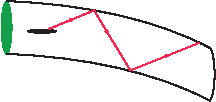
\includegraphics[width=2.5in]{photon-emission.pdf}}}$
\hspace{0.5in}
$\vcenter{\hbox{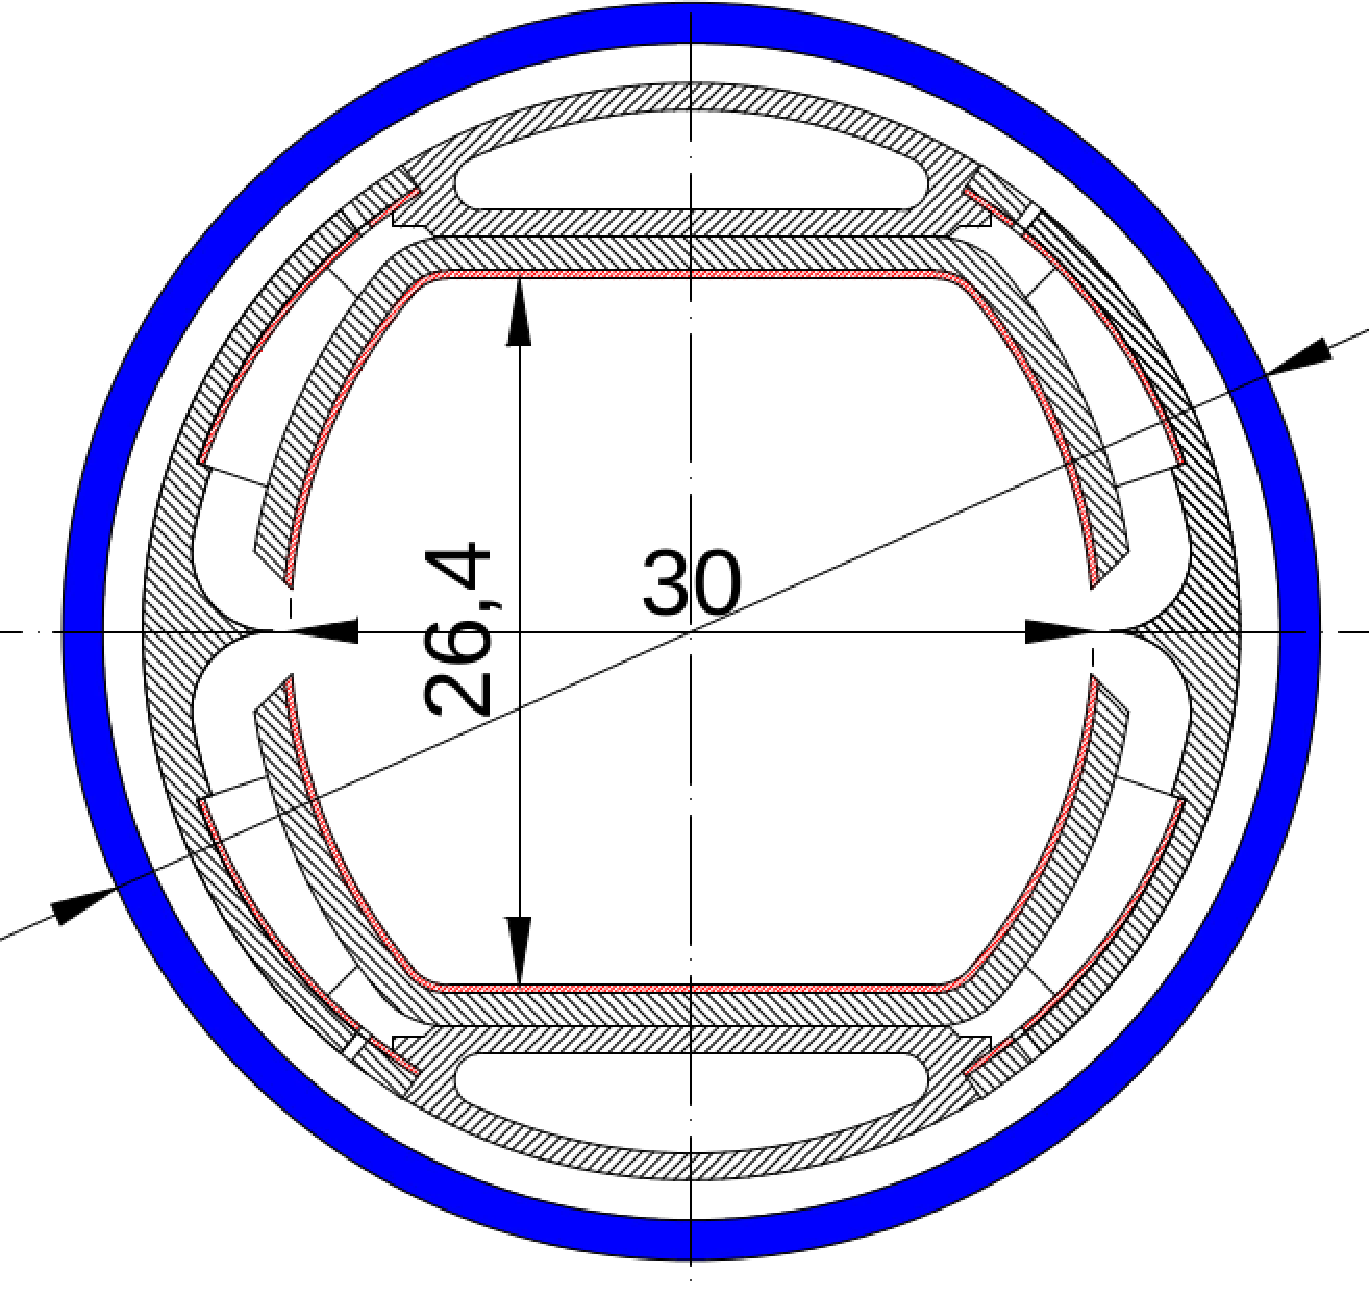
\includegraphics[width=2in]{lhc-cross-section.pdf}}}$

\vspace{1in}
{\Huge\bfseries Synrad3D Photon Tracking Program}

\vspace{0.4in}
{\LARGE\bfseries Gerry Dugan and David Sagan}

\vspace{0.4in}
{\large\bfseries December 5, 2017}

\end{center}
\end{titlepage}

\pdfbookmark[1]{Contents}{Contents}
\tableofcontents

%------------------------------------------------------------------
\chapter{Introduction} 
\label{s:intro}

\srthree is a program which simulates the production and scattering of
synchrotron radiation generated by an electron beam in a high energy
machine. The program was written by David Sagan and the photon
scattering model was developed by Gerry Dugan, both of Cornell
University.

\srthree is built atop the the Bmad software library
\cite{b:bmad}. The Bmad library, developed at Cornell, has been
developed for modeling relativistic charged particles in storage rings
and Linacs, as well as modeling photons in x-ray beam lines.

The motivation for developing \srthree was to estimate the energy and
position distribution of where SR photons are absorbed. This is a
critical input to codes which model the growth of electron clouds.
\srthree has also been used to model radiation mask efficiency.
\srthree includes scattering from the vacuum chamber walls, based on
X-ray data from an LBNL database~\cite{b:henke} for the smooth-surface
reflectivity, and an analytical model~\cite{b:beckmann,b:ogilvy} for
diffuse scattering from a surface with finite roughness. \srthree can
handle a wide variety of vacuum chamber profiles. \srthree also
handles a wide variety of machines including machines whose geometry
is not planar and machines using electrons or positrons as well as
machines using protons or antiprotons.

\srthree is not to be confused with an older program called
\vn{Synrad}. The \vn{Synrad} program is used for calculating wall
heating from the primary beam. \vn{Synrad} only tracks photons in the
horizontal plane and does not simulate the scattering of the photons
from the wall. The advantage of \vn{Synrad} is that it is fast and
directly gives wall heating numbers. The advantage of \srthree is that
it tracks photons in three dimensions and it does simulate scattering.

%------------------------------------------------------------------
\chapter{Running \srthree} 
\label{s:run}

Syntax for invoking \srthree:
\begin{example}
  synrad3d \{options\} \{<master_input_file_name>\}
\end{example}
Examples:
\begin{example}
  synrad3d my_input_file.init
  synrad3d -plot xy  my_input_file.init
\end{example}

The \vn{<master_input_file_name>} optional argument is used to set the
master input file name. The default is ``\vn{synrad3d.init}''. 

The command line options for \srthree are:
\begin{example}
  -plot <what>  ! For viewing diagnostic plots.
  -test <what>  ! For generating diagnostic files.
\end{example}

The \vn{-plot <what>} option is used for diagnostic purposes. When the
\vn{-plot} option is used, no photon tracking is done and instead a
plot window is displayed and \srthree will ask for the appropriate
parameters for making a plot. One of four types of plots is chosen by
the setting of \vn{<what>}:
\begin{example}
  -plot reflect ! Plot photon reflection probability curves.
  -plot xy      ! Plot cross-sections in the x-y plane.
  -plot xs      ! Plot cross-section in the x-s plane.
  -plot ys      ! Plot cross-section in the y-s plane.
\end{example}

The \vn{-plot reflect} option is for viewing photon reflection
probability curves. 

The \vn{-plot xy} option is for viewing of wall
cross-sections in the $x$-$y$ plane at any point in the machine. The
\vn{-plot xs} option plots the wall outline in the $x$-$s$ plane at $y
= 0$. The \vn{-plot ys} option plots the wall outline in the $y$-$s$
plane at $x = 0$. 

When plotting $x$-$s$ or $y$-$s$ cross-sections, if the Master Input file specifies a
\vn{photon_track_file}, this file will be read and the photon trajectories plotted.  If
the \vn{photon_track_file} does not exist, and a \vn{wall_hit_file} file does, the
\vn{wall_hit_file} will be read and the photon trajectories plotted. Since photon tracking
is {\em not} done when there is plotting done, the \vn{wall_hit_file} must be generated in
a previous run of \srthree prior to using the \vn{-plot} option.

When plotting $x$-$y$ cross-sections, symbols
will be drawn at the vertex points \vn{v(i)} that define the
cross-section.

The \vn{-test <what>} option is for generating diagnostic data. Tests are also useful for generating
data for plotting reflection statistics. Possible tests are:
\begin{example}
  -test monte_carlo_reflection ! \sref{s:test.monte}
  -test specular_reflection    ! \sref{s:test.specular}
  -test diffuse_probability    ! \sref{s:test.diffuse}
\end{example}
See Chapter \sref{s:test} for more details.

%------------------------------------------------------------------------
\chapter{Simulation Technique and Physics Models}
\section{Overview} 

The diffuse scattering theory used in \srthree is discussed by 
Dugan and Sagan\cite{b:prab} modified as discussed in \sref{c:spline}.

The \srthree program uses the Monte Carlo method for photon
generation, scattering, and absorption calculations.

For photon generation, a section of the machine (which may be the
complete machine) is designated for photon generation.  The total
number of photons generated is set by the user. \srthree calculates
how many photons need to be generated within each machine
element. Both circular and ``linear'' (that is, non-circular) machines
can be simulated.  In both cases, the orbit of the charged particle
beam, which may be non-zero, sets the centroid position and angular
orientation of the generated photons. The local bending field at the
beam orbit is used to determine the photon spectrum. Thus, for
example, radiation for an offset beam in a quadrupole is included.

The photon is tracked from the point of origin to
the point at which it hits the vacuum chamber wall. The angle of
incidence relative to the local normal to the vacuum chamber is
computed. A scattering probability is computed, based on this angle
and the photon's energy. Depending on the value of this probability,
the photon is either absorbed at this location, or scattered. If it is
scattered, the scattering is taken to be elastic. That is, photon
energy does not change. This ignores any florescence. Surface
roughness, on the other hand is taken into account so there is a
diffuse component to the scattering.

The photon is then tracked to the next encounter with the vacuum
chamber wall, and the probability of scattering is again
computed. This process continues until the photon is absorbed.

%------------------------------------------------------------------
\section{Photon Generation}

Photon generation is based on the standard synchrotron radiation
formulas, applicable for dipoles quadrupoles, and wigglers. The
radiation is assumed to be incoherent, so this program cannot treat
undulator radiation. Polarization of the photon is ignored.

\srthree slices up each element longitudinally
and generates photons from each slice. The number of photons generated
in a slice weighted by the local probability of photon emission which
depends on the local orbit curvature.

Both circular and ``linear'' (that is, non-circular) machines can be
simulated.  In both cases, the orbit of the charged particle beam,
which may be non-zero, sets the centroid position and angular
orientation of the generated photons. Photon generation is based upon
the local field along the beam orbit. Thus, for example, off-axis
photons in a quadrupole will produce radiation. The beam orbit is
calculated from such things as the settings of steering elements,
element misalignments, etc. as given in the lattice file. For circular
machines, the beam orbit is the closed orbit. For linear machines, the
starting beam position as set in the lattice file is used in the orbit
calculation.

When a photon is generated at a given longitudinal position, the
beam's emittances and centroid are used so that the resulting photon
distribution mirrors the Gaussian positional distribution of the beam.
Horizontal/vertical coupling is taken into account in this
calculation. The photon energy distribution will be the standard
energy spectrum of photons generated in a bend.

A photon's initial angular orientation is generated by first using a
random number generator to generate an angular orientation using a
probability function that corresponds to the beam's angular
distribution. To this orientation, an angular offset out of the plane
of the bend is added where the offset is calculated using a random
number generator with a probability distribution based on the standard
angular spectrum of photons generated in a bend. There is no angular
offset added to the angle in the plane of the bend. The generated
photons will have the proper correlation between photon energy and
photon angle. Note that the bending plane of the charged particle beam
need not be horizontal. For example, the bend plane orientation for an
offset beam in a quadrupole will depend upon the offset.

%------------------------------------------------------------------
\section{Photon Scattering} 

  \begin{figure}
  \centering
  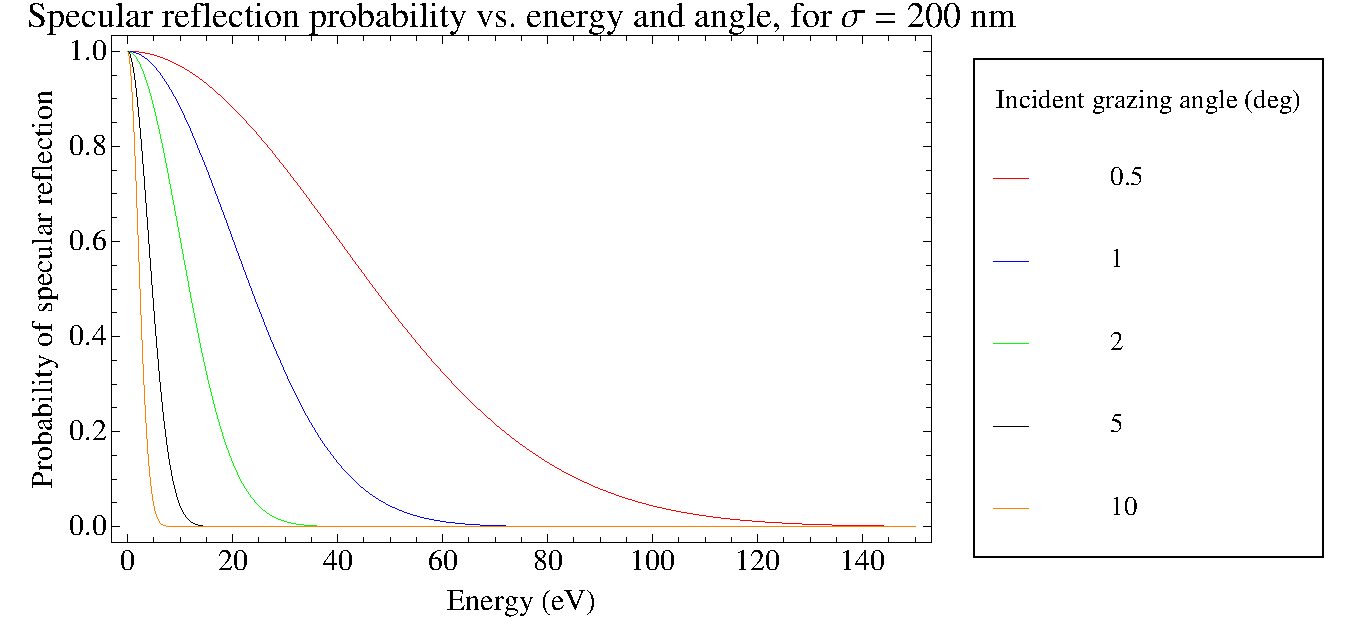
\includegraphics[width=6in]{specular-probability.pdf}
  \caption[Specular reflection probability vs. photon energy and angle]
{\label{f:spec.prob}
Specular reflection probability~\cite{b:beckmann}, vs. photon energy
and angle, for an rms surface roughness of 200 nm.}
  \end{figure}
   
Simulated photons are tracked until they hit the wall, where the
probability of being scattered, and the scattering angle, are
determined by their energy and angle of incidence.  This section
describes the scattering model.

Generally, the probability of specular reflection of a photon from a
rough surface depends on the the rms surface roughness $\sigma$, the
photon wavelength $\lambda$, and the grazing angle. An explicit
formula for this probability is~\cite{b:beckmann}
   \begin{equation}
P_{\textrm{spec}}=\textrm{e}^{-g(x,x)},
\end{equation}
in which
   \begin{equation}
g(x,y)=\frac{4\pi^{2}\sigma^{2}(x+y)^{2}}{\lambda^{2}}
  \end{equation}
where $x$ is the cosine of the incident polar angle, and $y$ is the
cosine of the scattered polar angle. For a typical technical vacuum
chamber surface, the rms surface roughness $\sigma \gtrsim 200$ nm is
greater than most of the X-ray wavelengths of interest, for all except
the lowest energy photons. In this regime, except at very small
grazing angles, diffuse scattering from the surface dominates over
specular reflection. This is illustrated in Fig.~\ref{f:spec.prob}.
The theory of diffuse scattering of electromagnetic waves from random
rough surfaces is a well-developed subject, and is covered in detail
in references \cite{b:beckmann} and \cite{b:ogilvy}. The model we use
assumes a Gaussian distribution for both the surface height variations
(rms $\sigma$) and for the transverse distribution (equal in both
transverse directions, with autocorrelation coefficient $T$).

  \begin{figure}
  \centering
  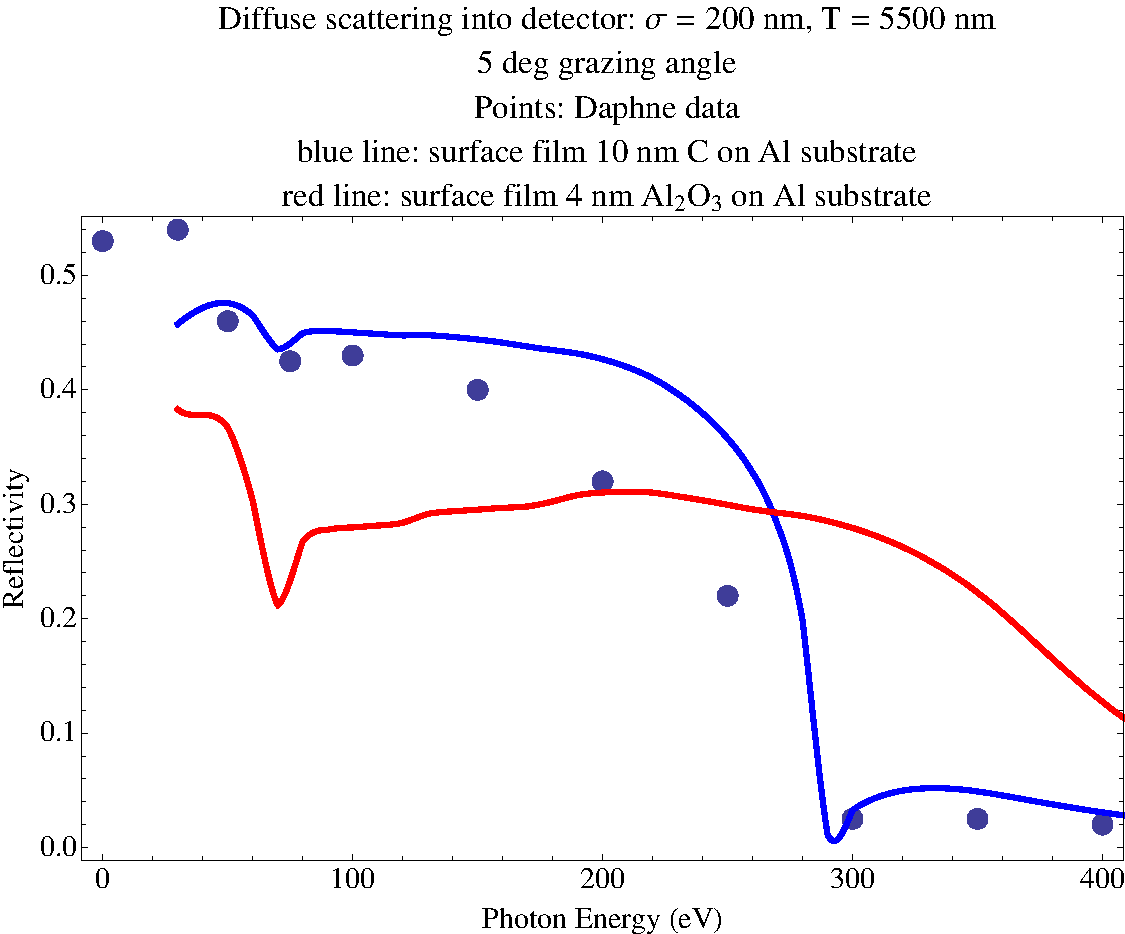
\includegraphics[width=4.5in]{Daphne-fit-5-deg}
  \caption{\label{f:Daphne.fit.5.deg}
   Diffuse scattering at 5 deg from a surface layer on an aluminum substrate: comparison of data and model}
   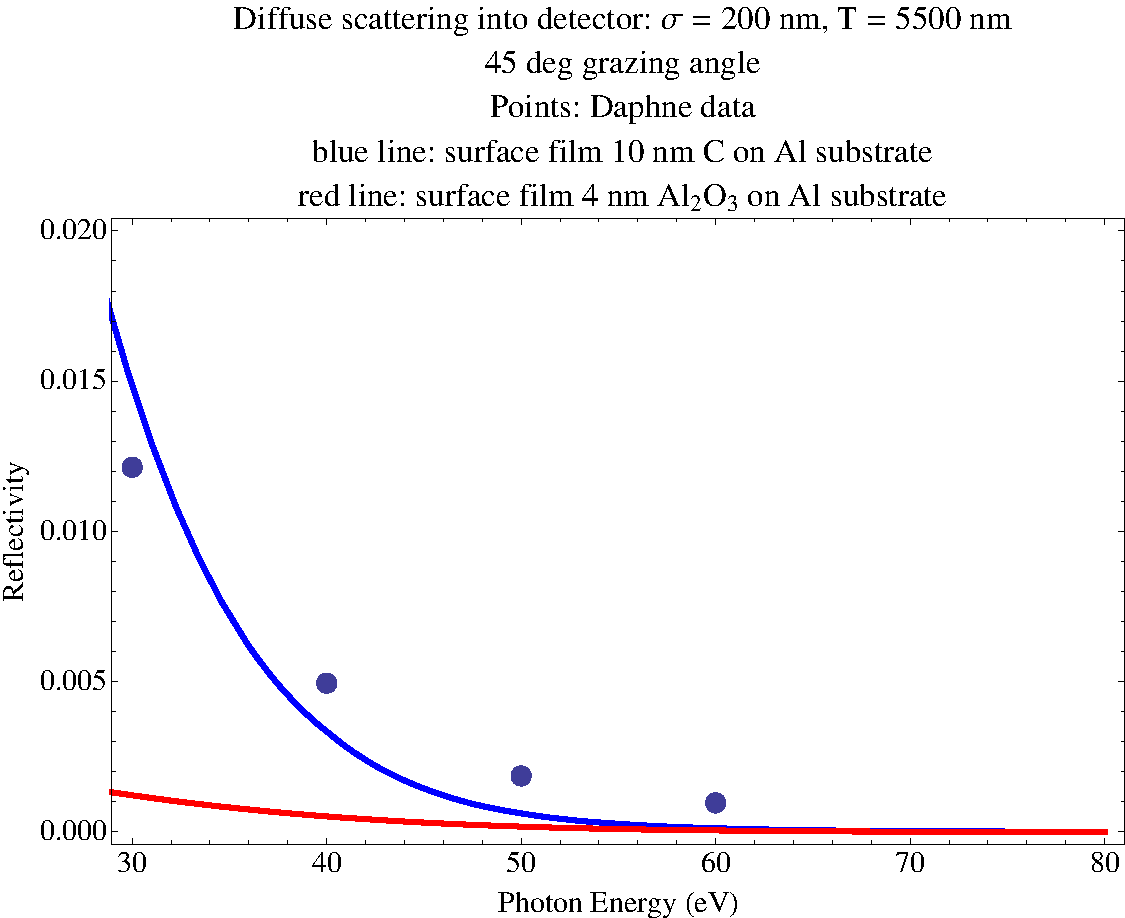
\includegraphics[width=4.5in]{Daphne-fit-45-deg}
   \caption{\label{f:Daphne.fit.45.deg}
   Diffuse scattering at 45 deg from a surface layer on an aluminum substrate: comparison of data and model}
   \end{figure}

  \begin{figure}
  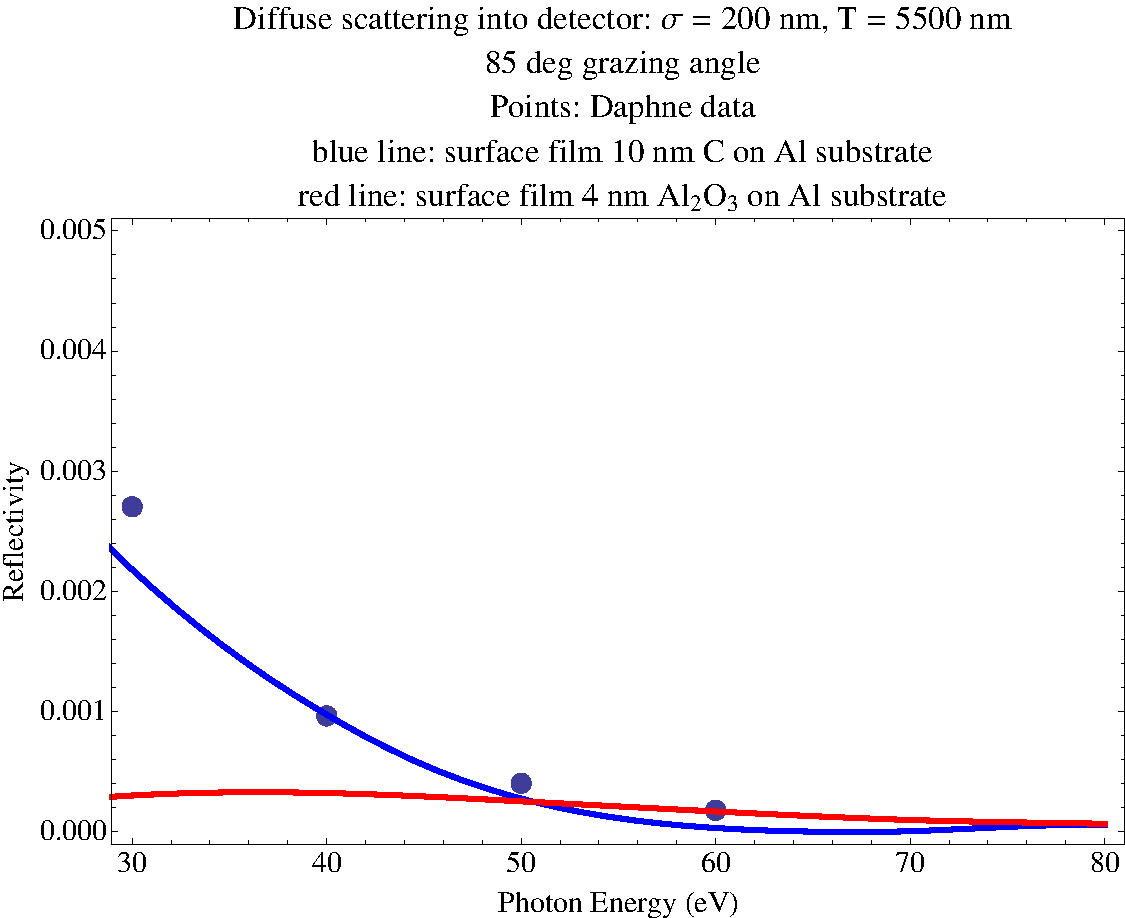
\includegraphics[width=4.5in]{Daphne-fit-85-deg}
   \caption{\label{f:Daphne.fit.85.deg}
   Diffuse scattering at 85 deg from a surface layer on an aluminum substrate: comparison of data and model}
  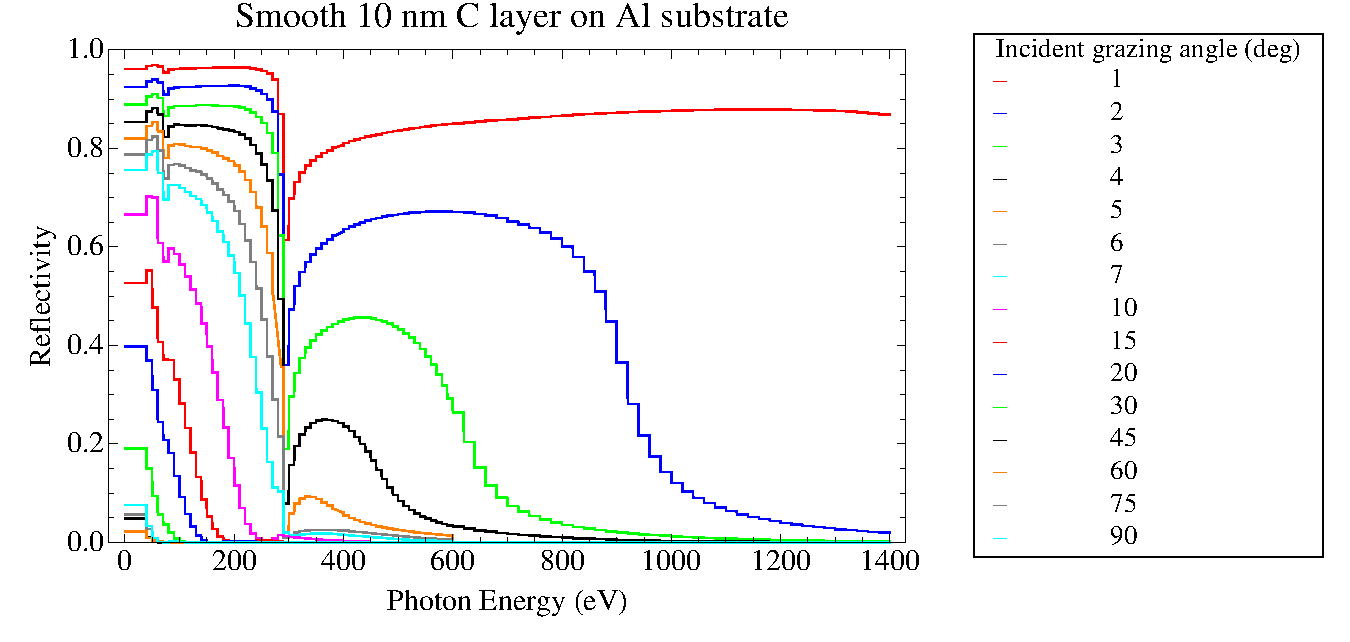
\includegraphics[width=6in]{Smooth-surface-reflectivity}
   \caption[Smooth surface reflectivity for a 10 nm C film on Al substrate]
   {\label{f:Smooth.surface.reflectivity}
   Smooth surface reflectivity for a 10 nm C film on Al substrate: from \cite{b:henke}}
  \centering
   \end{figure}

      \begin{figure}
  \centering
  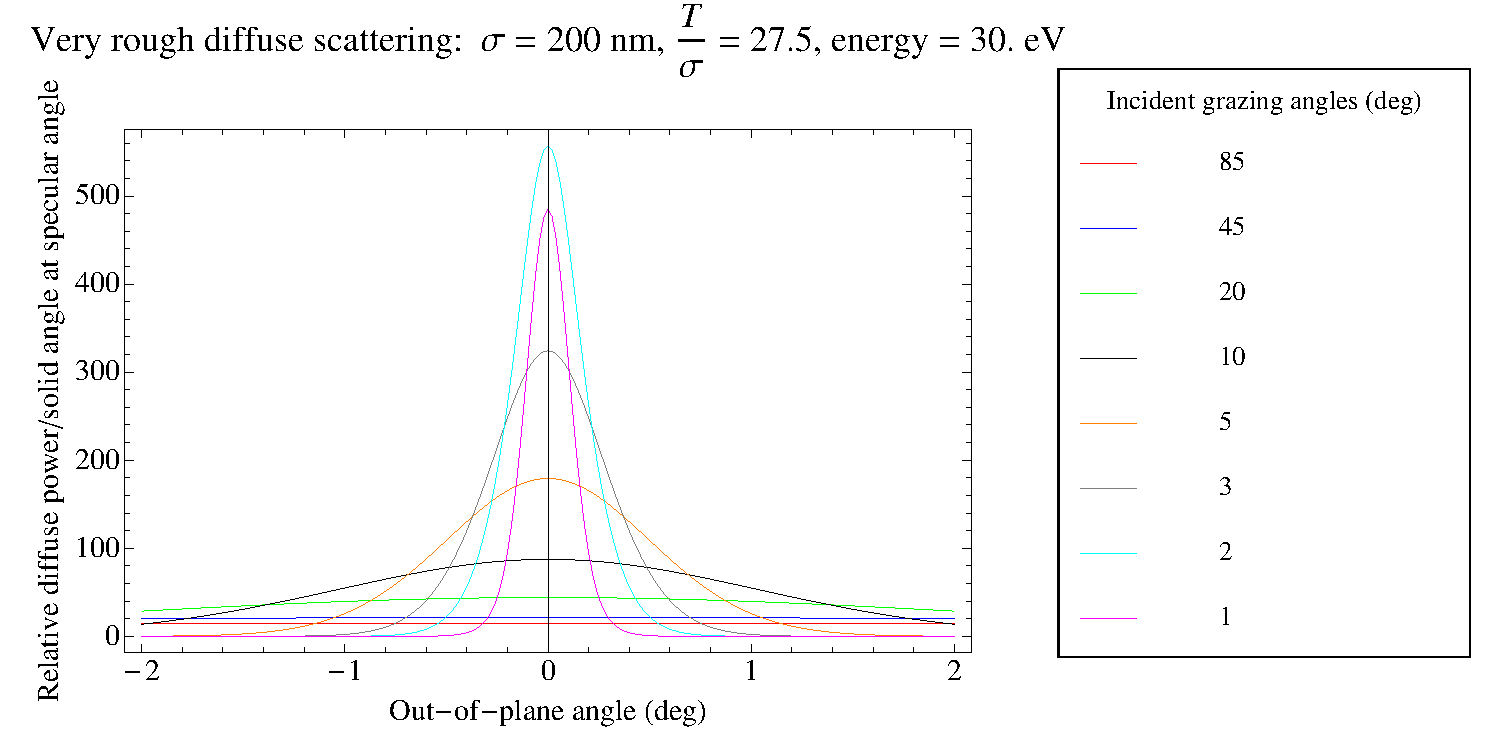
\includegraphics[width=6in]{Diffuse-out-of-plane-30ev}
   \caption{   \label{f:Diffuse.out.of.plane.30ev}
   Diffuse scattering out-of-plane angular distributions for 30 eV photons}
 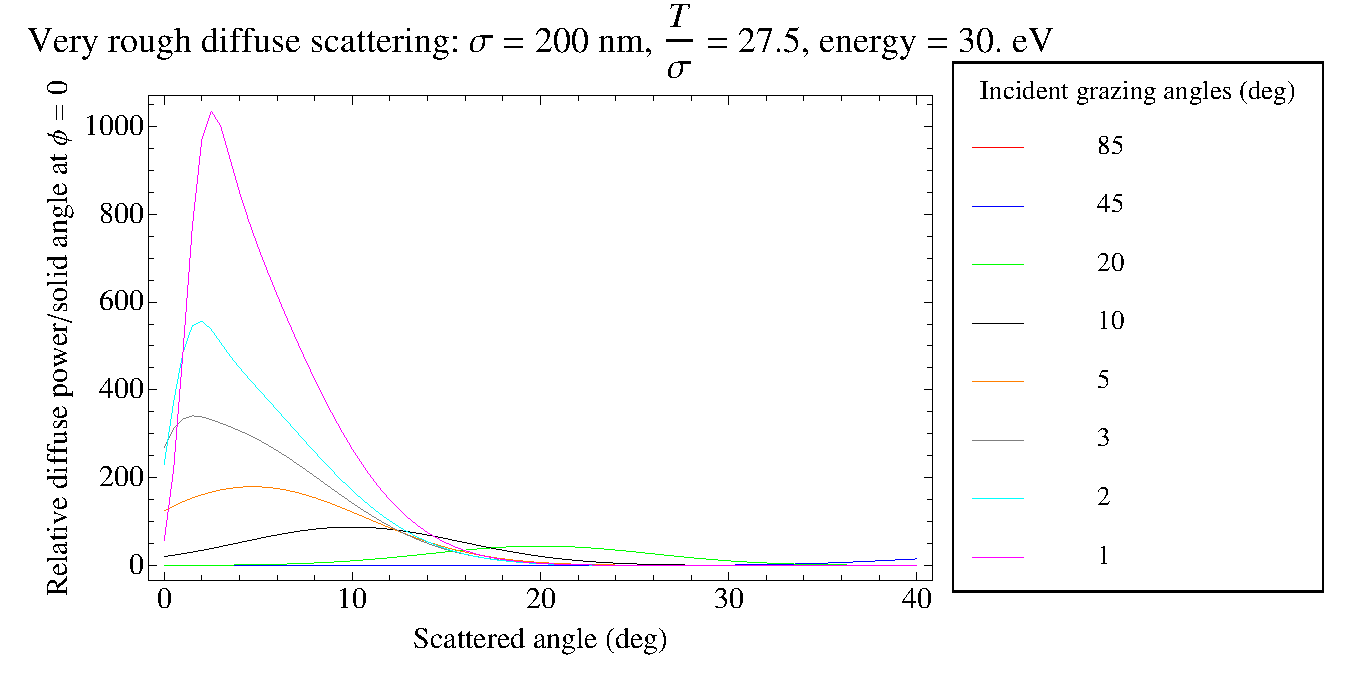
\includegraphics[width=6in]{Diffuse-polar-30ev}
   \caption{   \label{f:Diffuse.polar.30ev}
   Diffuse scattering polar angular distributions for 30 eV photons}
   \end{figure}

  \begin{figure}
  \centering
  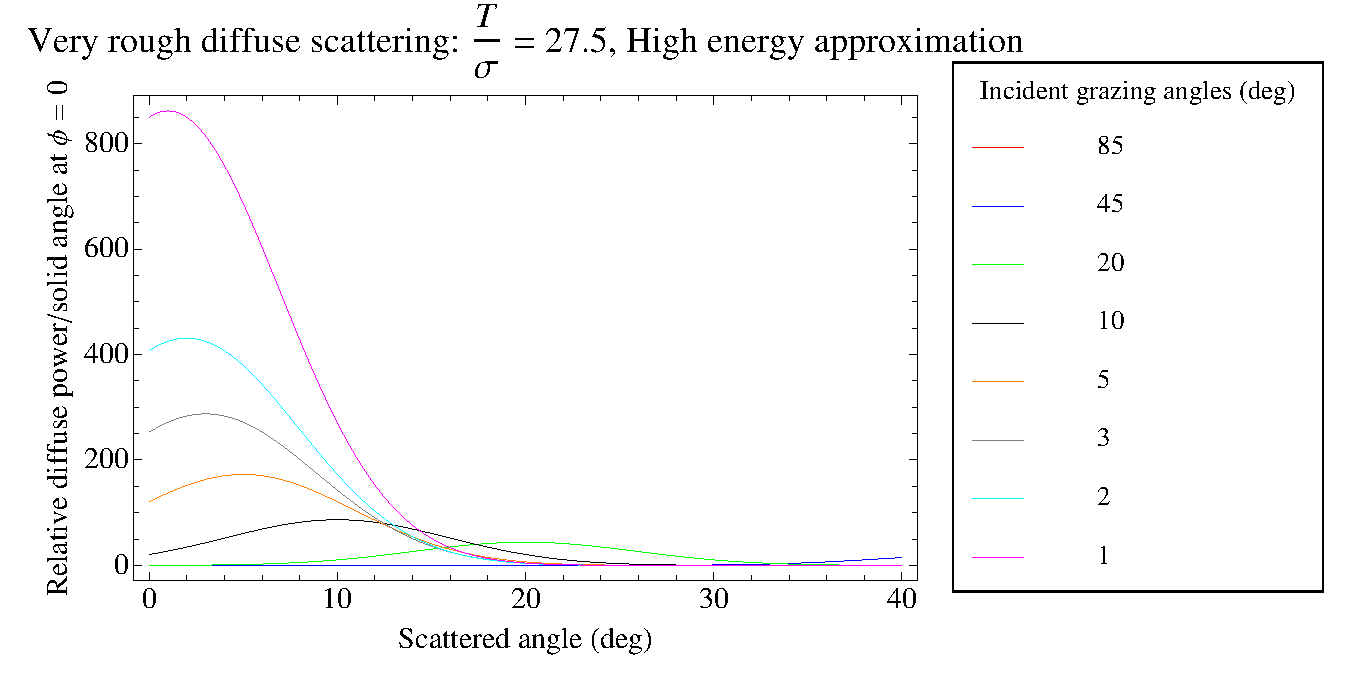
\includegraphics[width=6in]{Diffuse-polar-HE}
   \caption{   \label{f:Diffuse.polar.HE}
    Diffuse scattering polar angular distributions for high energy photons}
  \centering
  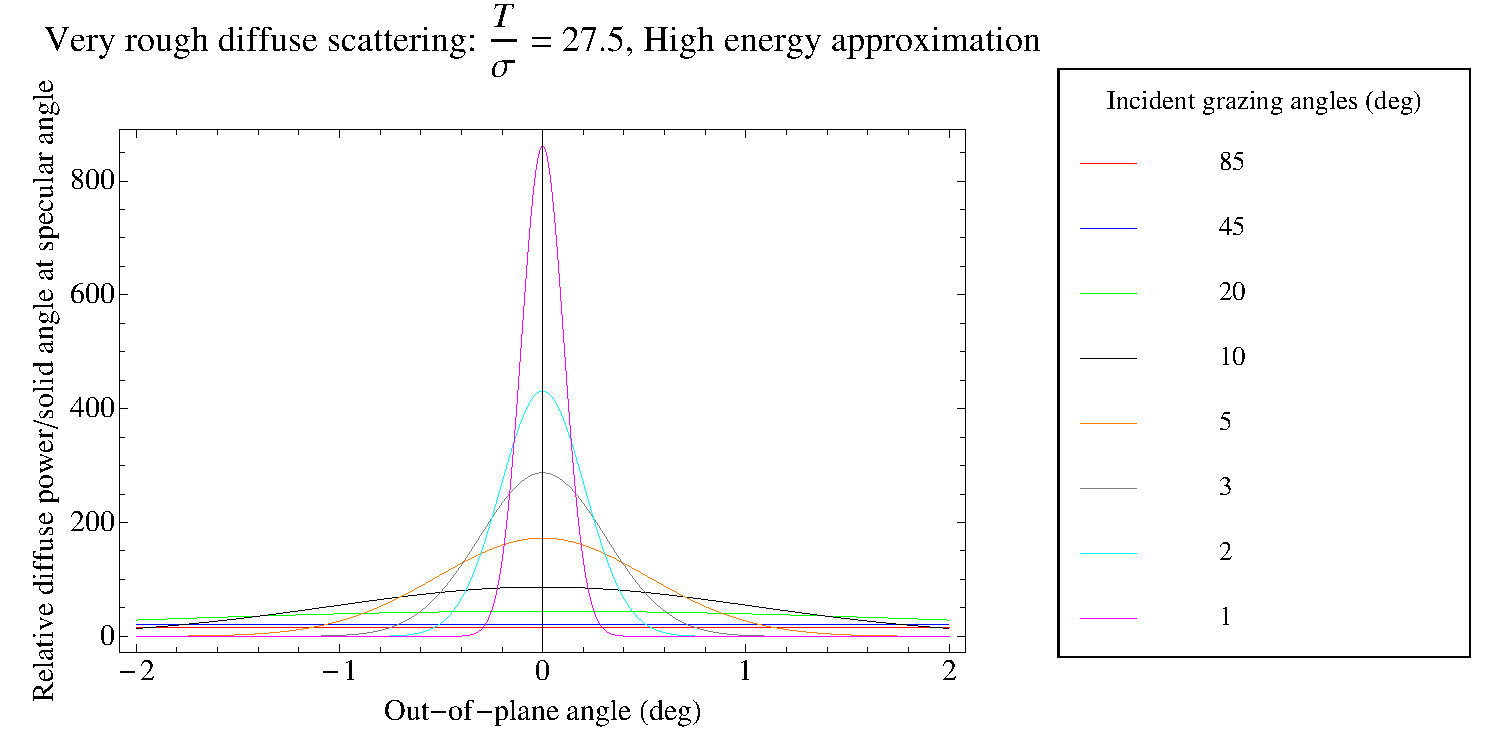
\includegraphics[width=6in]{Diffuse-out-of-plane-HE}
   \caption{   \label{f:Diffuse.out.of.plane.HE}
   Diffuse scattering out-of-plane angular distributions for high energy photons}
   \end{figure}
   
The most general expression for the diffusely scattered power is
complex, and involves an infinite sum.  However, the expression
simplifies substantially in the limit $g(x,y)\gg 1.$ For very rough
surfaces corresponding to technical vacuum chambers, for which
typically $\sigma \gg \lambda$, this condition is satisfied over much
of the region of interest. In this limit, the diffusely scattered
power per unit solid angle is given by
  \begin{equation}
  \frac{d P_{\textrm{diff}}}{d \Omega} = P_{0}\frac{\left<R\right>}{4\pi y}
  \frac{(1+xy)^{2}}{(x+y)^{4}}\tau^{2}\textrm{e}^{-\frac{(2-x^{2}-y^{2})
  \tau^{2}}{4(x+y)^{2}}}(1-a\cos\phi)^{2}\textrm{e}^{b\cos\phi},
  \label{Eq.diffuse.power}
  \end{equation}
with
   \begin{align}
   a&=\frac{h(x,y)}{1+xy}, \\
   b&=\frac{2h(x,y)\tau^{2}}{4(x+y)^{2}}, \\
   h(x,y)&=\sqrt{1-(x^{2}+y^{2})+x^{2}y^{2}}.
   \end{align}
In this expression, $P_{0}$ is the incident power, and
$\left<R\right>$ is the smooth-surface reflectivity, which is
determined by the atomic structure of the surface material. $\phi$ is
the scattering angle out of the plane of incidence. Note that the
relative power depends on the ratio $\tau=T/\sigma$, and not on the
$T$ or $\sigma$ separately.

The smooth-surface reflectivity $\left<R\right>$ depends on the atomic
structure of the surface materials (including any thin layers which
may be deposited on the surface). The surface roughness parameters
$\sigma$ and $T$ depend on the geometry of the surface deviations from
a perfect plane. These parameters may be determined from inspection of
the vacuum chamber surface, for example, using an atomic force
microscope.

To derive a working model for the smooth surface reflectivity and the
surface parameters for a typical vacuum chamber surface, we have
relied on measurements~\cite{b:mehne} of X-ray scattering
from an aluminum vacuum chamber surface made at \vn{DAPHNE}. For
these measurements, the rms surface roughness of the sample was
reported to be 200 nm.

The theory of diffuse scattering discussed above has been used,
together with smooth surface reflectivity results taken from an X-ray
database~\cite{b:henke}, to predict the scattering and compare with
the measurements. From these comparisons, the best-fit value for the
transverse autocorrelation parameter, $T$, was found to be 5500 nm. As
discussed by Dugan and Sagan\cite{b:synrad3d},
it was found that the smooth-surface reflectivity
corresponding to a 10 nm carbon film on an aluminum substrate was
needed to fit the data. The assumption of an aluminum oxide surface
film was not consistent with the data. The data and the corresponding
fits are shown in Fig.~\ref{f:Daphne.fit.5.deg},
\ref{f:Daphne.fit.45.deg}, and \ref{f:Daphne.fit.85.deg}.

With the smooth-surface reflectivity determined, and the surface
parameters established, the scattering model in \srthree is
completely determined. The model currently in use has a smooth-surface
reflectivity illustrated in
Fig.~\ref{f:Smooth.surface.reflectivity}. Diffuse
scattering distributions for 30 eV photons are shown in
Fig.~\ref{f:Diffuse.polar.30ev} and
Fig.~\ref{f:Diffuse.out.of.plane.30ev}. At this low photon
energy, the approximation $g(x,y)\gg 1$ does not hold in general, and
the full diffuse scattering formalism is used to compute these
distributions. Diffuse scattering distributions for high energy
photons, for which $g(x,y)\gg 1$ are shown in
Fig.~\ref{f:Diffuse.polar.HE} and
Fig.~\ref{f:Diffuse.out.of.plane.HE}. These distributions
have been computed from Eq.~\ref{Eq.diffuse.power}.

%------------------------------------------------------------------
\chapter{Master Input File} 
\label{s:master}

%------------------------------------------------------------------
\section{Fortran Namelist}
\label{s:namelist}

Fortran namelist syntax is used for parameter input by \srthree. The
general form of a namelist is
\begin{example}
  &<namelist_name>
    <var1> = ...
    <var2> = ...
    ...
  /
\end{example}
The tag \vn{"\&<namelist_name>"} starts the namelist where
\vn{<namelist_name>} is the name of the namelist. The namelist ends
with the slash \vn{"/"} tag. Anything outside of this is
ignored. Within the namelist, anything after an exclamation mark
\vn{"!"} is ignored including the exclamation mark. \vn{<var1>},
\vn{<var2>}, etc. are variable names. Example:
\begin{example}
  &place section =   0.0, "arc_std", "elliptical", 0.045, 0.025 /
\end{example}
here \vn{place} is the namelist name and \vn{section} is a
variable name.  Notice that here \vn{section} is a ``structure'' which
has five components -- a real number, followed by two strings,
followed by two real numbers.

Everything is case insensitive except for quoted strings.

Logical values are specified by \vn{True} or \vn{False} or can be
abbreviated \vn{T} or \vn{F}. Avoid using the dots (periods) that one
needs in Fortran code.

%------------------------------------------------------------------
\section{Example Master Input File} 
\label{s:master.example}

The master input file can be specified on the command line invoking \srthree.
If not given, the default name for the master input file is ``\vn{synrad3d.init}''.

Fortran namelist syntax is used (\sref{s:namelist}). Example master input file:
\begin{example}
  &synrad3d_parameters
    ix_ele_track_start   = 1      ! Radiation region start lattice element.
    ix_ele_track_end     = 912    ! Radiation region end lattice element.
    photon_direction     = 1      ! 1 = Forward generation, -1 = Backward generation.
    num_photons          = 50000  ! Target number of unfiltered photons.
    num_photons_per_pass = -1     ! Number of photons generated per pass. -1 = Use num_photons/5.
    ds_step_min          = 0.01   ! Photons are generated at discrete points. 
                              ! Multiple photons can be generated at each point.
                              ! This is minimum distance between points.
    emit_a       = -1         ! Horizontal emit. Meters. If < 0 -> Calc from lattice.
    emit_b       = 7.52E-11   ! Vertical emit.  Meters. If < 0 -> Calc from lattice.
    sig_e        = -1         ! Sig_E/E. If < 0 -> Calc from lattice.

    lattice_file = "../lattice/cesr/bmad/bmad_6wig_8nm_2085.lat" 
    wall_file    = "synrad3d.wall"   ! Vacuum chamber wall file.
    dat_file     = "synrad3d.dat"    ! Output data file.
    wall_hit_file = ""               ! Photon wall hit output data file.
    photon_track_file = ""           ! Photon track output data file
    lat_ele_file  = ""               ! Write lattice element data file.
    photon_start_input_file  = ""    ! File for initializing the photons
    photon_start_output_file = ""    ! File recording photon start positions

    random_seed = 123456             ! 0 -> Use sys clock.
    e_init_filter_min = -1           ! Min initial energy filter param.
    e_init_filter_max = -1           ! Max initial energy filter param.
    e_filter_min = -1                ! Min final energy filter param.
    e_filter_max = -1                ! Max final energy filter param.
    s_filter_min = -1                ! Min S position filter param.
    s_filter_max = -1                ! Max S position filter param.
    filter_phantom_photons = T       ! Filter photons striking a phantom wall?
    num_ignore_generated_outside_wall = 0    !
    turn_off_kickers_in_lattice = F          ! Zero the closed orbit?
    surface_roughness_rms       = -1         ! Surface roughness for diffuse scattering.
    roughness_correlation_len   = -1         ! Surface roughness correlation length.
    surface_reflection_file     = ""         ! File for specifying default reflection probabilities.
    chamber_end_geometry = ""                   ! For defining the wall at the ends of the lattice
    sr3d_params%ds_track_step_max        = 3    ! Photon propagation step size 
    sr3d_params%dr_track_step_max        = 0.1  ! Photon propagation step size 
    sr3d_params%specular_reflection_only = F    ! For testing the effect of diffuse scattering.
    sr3d_params%allow_reflections        = T    ! For testing purposes.
    sr3d_params%allow_absorption         = T    ! For testing purposes.
  /
\end{example}

  \begin{description}
  \item[\vn{ds_step_min}] \Newline
This parameter establishes the minimum distance to track the particle beam between emission
points. The thought was that if \srthree decided to make very small steps  between emission
points, this might slow the calculation down. This has not been tested. This parameter
does not influence photon tracking.
  \item[\vn{ix_ele_track_start}, \vn{ix_ele_track_end}] \Newline
The parameters \vn{ix_ele_track_start} and \vn{ix_ele_track_end} establish
the region where radiation is produced. These are the index numbers of 
elements in the lattice. The radiation region boundary is taken to be at
the exit end of the elements so no radiation is produced in the element
with index \vn{ix_ele_track_start}. If \vn{ix_ele_track_end} is negative,
the end of the radiation region is taken to be end of the lattice.
If \vn{ix_ele_track_end} is positive and less than \vn{ix_ele_track_start},
the track region will be from \vn{ix_ele_track_start} through the
end of the lattice and from the beginning of the lattice to \vn{ix_ele_track_end}.
  \item[\vn{photon_direction}] \Newline
The \vn{photon_direction} parameter determines in what direction the photons
are traveling when initially created. A value of \vn{+1} indicates the photons
are created traveling in the $+s$ direction and a value of \vn{-1} indicates
that the photons are created in the $-s$ direction.
  \item[\vn{num_photons}] \Newline
\vn{num_photons} establishes the minimum number of ``unfiltered''
photons that need to be generated before \srthree will stop the
simulation. The actual number of unfiltered photons will be between
\vn{num_photons} and \vn{num_photons+num_photons_per_pass} See
below for more details. [An unfiltered photon is a photon that passes
all filter requirements and is recorded in the output statistics.]
  \item[\vn{num_photons_per_pass}] \Newline
\vn{num_photons_per_pass} sets the number of photons generated per
``pass''.  A ``pass'' is the act of generating photons throughout the
radiation production region. If \vn{num_photon_per_pass} is negative
(the default), the number of photons generated per pass is taken
to be \vn{num_photons}/5. The actual number of unfiltered photons will be between
\vn{num_photons} and \vn{num_photons+num_photons_per_pass} See
below for more details.
  \item[\vn{emit_a}, \vn{emit_b}, \vn{sig_e}] \Newline
These parameters set the particle beam size and so will affect the starting coordinates of
the photons. A negative set of any of these parameters will result in \srthree 
using the value for the parameter from a calculation of the synchrotron radiation integrals.
  \item[\vn{lattice_file}] \Newline
This file defines the machine optics. The lattice file format may be
the Bmad format or, if the \vn{lattice_file} string is prefixed by
\vn{``xsif::''}, may be in xsif format. See the Bmad manual for more details.
  \item[\vn{photon_track_file}] \Newline
This string, if not blank, will create a data file with a table of points along the photon tracks.
This file is useful for plotting photon trajectories since it records intermediate points between
points where the photon hits a wall.
See \sref{s:photon.track.file} for more details
  \item[\vn{wall_file}] \Newline
This string gives the name of the vacuum chamber wall definition
file. See \sref{s:wall.file} for more details.
  \item[\vn{dat_file}] \Newline
This string gives the name of the output data file (\sref{s:main.out}).
See below for more details.
  \item[\vn{surface_roughness_rms}] \Newline
This parameter sets the surface roughness RMS in meters for the
default surface (\sref{s:dflt.reflect}). This is used for diffuse
scattering.  If negative (the default), the value 200~nm will be used.
  \item[\vn{roughness_correlation_len}] \Newline
This parameter sets the surface roughness correlation length in meters
for the default surface (\sref{s:dflt.reflect}).  This is used for
diffuse scattering.  If negative (the default), the value of
5.5~$\mu$m will be used.
  \item[\vn{surface_reflection_file}] \Newline
This parameter is used to change the default reflection probability curves used in the
simulation. See \sref{s:reflect.file} for details. To define multiple surfaces with
differing reflectivities, see \sref{s:surface}.
  \item[\vn{sr3d_params\%allow_reflections}] \Newline
This parameter, if set False, will cause \srthree to stop tracking a given photon once
it hits the chamber wall. This can be used to generate data on where the primary photons are striking.
  \item[\vn{sr3d_params\%specular_reflection_only}] \Newline
This parameter can be used to test whether diffuse scattering is important. If set to \vn{True},
photons will always be specularly reflected. Default is \vn{False}.
  \item[\vn{sr3d_params\%allow_absorption}] \Newline
This parameter, if set False, will cause \srthree suppress absorption
and to always reflect photons when they hit the chamber wall. This
parameter is only used for testing purposes.
  \item[\vn{sr3d_params\%ds_track_step_max}, \vn{sr3d_params\%dr_track_step_max}] \Newline
These parameters determine the maximum distance a photon is tracked in
a given ``step'' see \sref{s:track} for more details.
  \item[\vn{wall_hit_file}] \Newline
This string, if not blank, will create a data file listing the points
where the photons hit the wall including all the reflection
points. This will be in addition to the regular output file.  See
\sref{s:wall.hit.file} for more details.
  \item[\vn{lat_ele_file}] \Newline
This string, if not blank, will create a data file listing  the lattice
elements within the emission region. For each element the following are given. 
  \begin{enumerate}
  \item
    The element name
  \item
    The element type (quadrupole, etc.)
  \item
    Longitudinal position at the exit end of the element
  \item
    Element length.
  \item
    $I_0$ radiation integral through the element.
  \item
    The nominal (not actual) number of photons to be generated based upon the $I_0$ integral,
    the total $I_0$ integral, and the setting of \vn{num_photons}
  \item
    The longitudinal step size between photon emission points.
  \end{enumerate}

  \item[\vn{random_seed}] \Newline
Random number seed used in by the random number generator. If set to 0, the system clock
will be used. That is, if set to 0, the output results will vary from run to run. 
  \item[\vn{e_init_filter_min}, \vn{e_init_filter_max}] \Newline
Minimum and maximum initial energy filter values. A negative filter value
indicates that the particular filter is not used. See below.
  \item[\vn{e_filter_min}, \vn{e_filter_max}] \Newline
Minimum and maximum energy filter values. A negative filter value
indicates that the particular filter is not used. See below.
  \item[\vn{s_filter_min}, \vn{s_filter_max}] \Newline
Minimum and maximum longitudinal position filter values of the final
photon position. A negative filter value indicates that the particular
filter is not used. See below.
  \item[\vn{filter_phantom_photons}] \Newline
Phantom photons are photons that have hit a ``phantom'' wall (\sref{s:surface}).  That is,
a wall whose surface name is set to ``PHANTOM''. If \vn{filter_phantom_photons} is set the
\vn{True} (the default) a filter test is used to exclude phantom photons from the output.
If set to \vn{False}, the filter will not be applied.
  \item[\vn{photon_start_output_file}] \Newline
This string, if not blank, will cause \srthree to create an output file, with a name given
by the value of \vn{photon_start_output_file}, of the photon starting positions along with
the state of the random number generator. The format for this file is compatible with the
format of the \vn{photon_start_input_file}. This file is generally used for debugging
purposes and is not of general interest. Note: If \vn{photon_start_input_file} is set,
\vn{photon_start_output_file} will be ignored (no output file is generated). Also note
that the file will have the starting coordinates of all photons generated, not just the
photons that pass any filtering tests. Thus, if any of the filter parameters are set, the
size of the file may be very large. See below for the syntax of this file.
  \item[\vn{photon_start_input_file}] \Newline
If not blank, the file named by \vn{photon_start_input_file} will be read by \srthree and
used to initialize photon starting positions. See \sref{s:photon.start} for the syntax of
this file.  The state of the random number generator at the time of a photon's
initialization can also be specified in the file. In this case, the random number
generator state will also be set along with the state of the photon. This is useful for
diagnostic purposes when one wishes to compare the results of different versions of the
\srthree program. The syntax for this file is the same as the syntax used to generate the
\vn{photon_start_output_file}. See below for the syntax of this file.

If \vn{photon_start_input_file} is set to ``\vn{CUSTOM}'', instead of reading from a file, custom
code is used to generate the initial photon position. Details of how this works is given
in Sec.~\sref{c:custom}.
  \item[\vn{num_ignore_generated_outside_wall}] \Newline
Photons may be generated outside of the beam chamber for various
reasons. For example, the beam chamber can be too small or the closed
orbit may lie near or outside the chamber. Another possibility is that
the beam emittance is large enough so that, from time-to-time, a
photon generated at large amplitude will be generated outside the
wall. \srthree will ignore photons generated outside the wall, and
generate another one at the same longitudinal position, up to the
number set by \vn{num_ignore_generated_outside_wall}. If the number of
photons generated outside the wall exceeds this number, \srthree will
print an error message and stop.
  \item[\vn{turn_off_kickers_in_lattice}] \Newline
If \vn{turn_off_kickers_in_lattice} is set to True (the default is
False), then all kicks from steering elements in the lattice will be zeroed.
  \item[\vn{chamber_end_geometry}] \Newline
The \vn{chamber_end_geometry} sets how the chamber ends at the ends of the lattice
are treated. \vn{chamber_end_geometry} may be set to one of:
\begin{example}
  ""            ! Use lattice geometry
  "closed"      ! The chamber ends connect together.
  "open"        ! The chamber end are not connected together.
\end{example}
If \vn{chamber_end_geometry} is set to blank (""), the setting of the lattice geometry
will be used as the chamber geometry (the lattice geometry is set in the lattice file, see
the Bmad manual\cite{b:bmad} for more details). For a \vn{"closed"} geometry, the chamber
ends at the ends of the lattice are connected together so a photon hitting one end will
reappear at the other end.  For an \vn{"open"} geometry, the camber ends at the ends of
the lattice are not connected so a photon hitting an end will be reflected or absorbed.

Note: the setting of \vn{chamber_end_geometry} only affects branch 0 (the root branch) of
the lattice. If The lattice has other branches, the chamber end geometry for chambers in
these branches is always determined by the \vn{geometry} setting for the branch.
\end{description}

\srthree will generate a set of approximately \vn{num_photons_per_pass} photons in the
radiation production region.  This is called a ``pass''.  After any filtering, \srthree
will check to see if the number of unfiltered photons is at least \vn{num_photons}.  If
so, photon generation will stop. If not enough photons have been generated, \srthree will
generate another \vn{num_photons_per_pass}, and so on, until at least \vn{num_photons}
unfiltered photons have been generated. Thus the actual number of unfiltered photons
will be between \vn{num_photons} and \vn{num_photons_per_pass}.

The six "filter" parameters are:
\begin{example}
  e_init_filter_min   ! min initial energy filter.
  e_init_filter_max   ! max initial energy filter.
  e_filter_min        ! min energy filter.
  e_filter_max        ! max energy filter.
  s_filter_min        ! min longitudinal position filter.
  s_filter_max        ! max longitudinal position filter.
\end{example}
A filter parameter is "unset" if its value is negative and is "set"
otherwise.

Photons that do not satisfy the set filter values are discarded. The
\vn{e_init_filter_min} and \vn{e_init_filter_max} parameters are 
compared against the initial photon energy, and the other four
filter parameters are compared against the final photon position and
energy. The s-filter can wrap around $s = 0$: That is,
if both \vn{s_filter_min} and \vn{s_filter_max} have been set,
and \vn{s_filter_min} is {\em greater} than \vn{s_filter_max}, the region
for keeping a photon is from \vn{s_filter_min} through the end of the
lattice along with the region from the start of the lattice to
\vn{s_filter_max}.

Note: Processes like florescence can create photons with an energy that is different
from the energy of the photon that initiates the process. \srthree does not model such
processes so the final photon energy will be equal to the initial photon energy. This
being the case, \vn{e_init_filter_min} and \vn{e_init_filter_max} are equivalent to
\vn{e_filter_min} and \vn{e_filter_max} respectively. Furthermore, the execution time of a
simulation will be speeded up if \vn{e_init_filter_min} and \vn{e_init_filter_max} are
used instead of \vn{e_filter_min} and \vn{e_filter_max} since less tracking will be done.

%------------------------------------------------------------------
\chapter{Vacuum Chamber} 
\label{s:vac.chamber}

\begin{figure}[bt]
\begin{center}
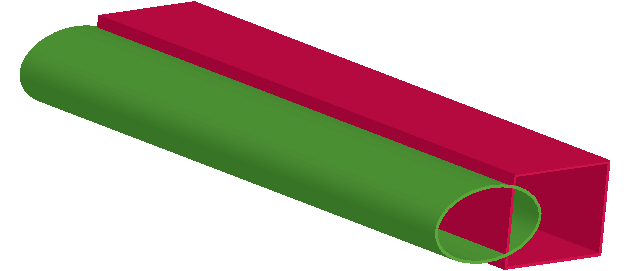
\includegraphics[width=5in]{vac-pipe.pdf} \caption[The vacuum chamber is the union of a
number of subchambers.]{The vacuum chamber is the union of a number of subchambers.
This figure illustrates this showing two subchambers -- one colored green and the other
colored red. A photon is considered within the vacuum chamber if, and only if, it is
inside at least one of the subchambers.}
\label{f:vac-chamber}
\end{center}
\end{figure}

%------------------------------------------------------------------
\section{Subchambers}
\label{s:sub.chambers}

The shape of the vacuum chamber is described by a number of ``subchambers'' (the reason
for dividing the vacuum chamber into subchambers is discussed in \sref{s:track}). This is
illustrated in \fig{f:vac-chamber}. The entire vacuum chamber is the union of all the
subchambers. That is, a photon is considered within the vacuum chamber if, and only if,
it is inside at least one of the subchambers. It is perfectly fine for subchambers to
overlap one another. In fact, some overlap is desirable to prevent abutting subchambers
from appearing to be separated due to round-off errors in the calculation.

%------------------------------------------------------------------
\section{Wall_file Syntax}
\label{s:wall.file}

The vacuum chamber is defined in the \vn{wall_file}. The name of the \vn{wall_file} is
specified in the master input file \sref{s:master}. The syntax for specifying the vacuum
chamber follows Fortran namelist input as explained in \sref{s:namelist}.

  \begin{figure}[tb]
  \begin{center}
  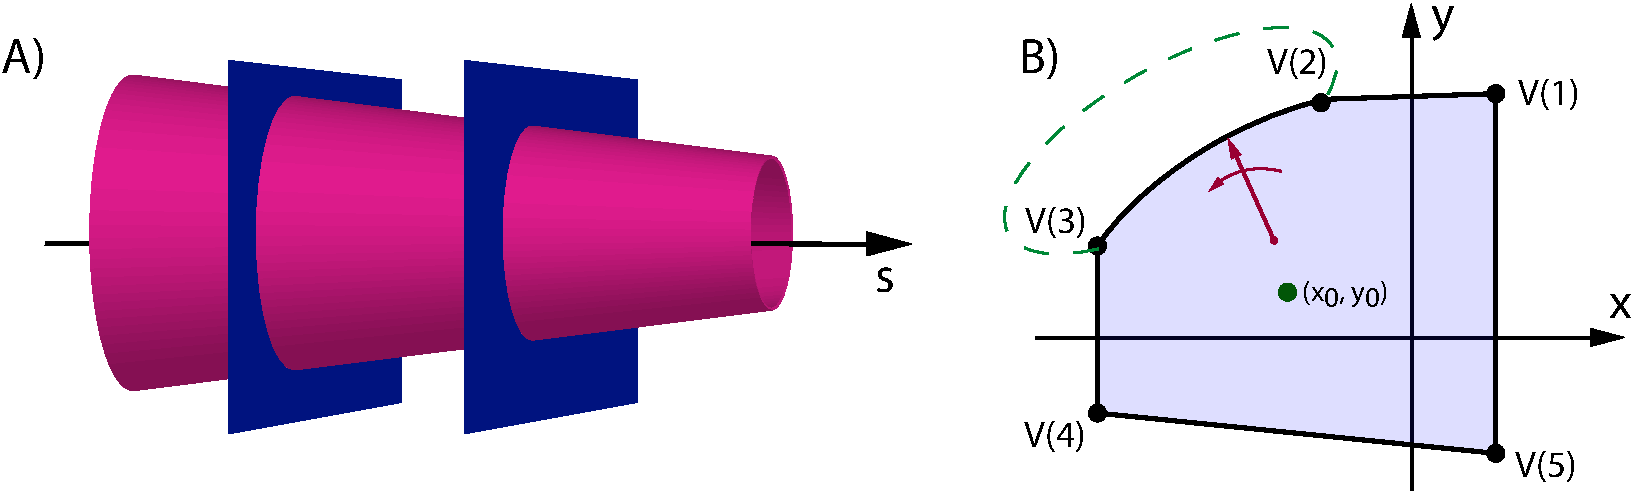
\includegraphics[width=6in]{chamber-wall.pdf} 
\caption{A subchamber is defined by a number of cross-sectional slices. A) A subchamber
(red) and two cross-sectional slices (blue). B) A given cross-section is defined by a
number of vertices.}
  \label{f:chamber.wall}
  \end{center}
  \end{figure}

Each subchamber is defined by specifying the subchamber cross-section at
a number of longitudinal positions as illustrated in
\fig{f:chamber.wall}. Each cross-section is specified using a namelist
named \vn{place}. The general form of a \vn{place} namelist is:
\begin{example}
  &place 
    section = <s>, "<section_name>", "<section_id>" 
    surface = "<surface_name>", <is_local>
  /
\end{example} 
The optional \vn{surface} parameter, which is used to specify a particular surface, is
explained in \sref{s:surface}.  Example:
\begin{example}
  &place section =   0.0, "arc_std", "beam:dipole_shape" /
  &place section =  74.3, "Near_IR"  "left_ante:shape-A@START" /
  &place section =  82.9, "wig1",    "left_ante:shape-B@END"
  &place section =  91.1, "IR1",     "rectangle" /
\end{example}

The \vn{<s>} values for the cross-sections of a given subchamber must
be in increasing order and there must be one subchamber that has a
cross-section at \vn{<s>} = 0. If the last cross-section of a given
subchamber has \vn{<s>} greater than the end of the lattice, the
\vn{<s>} value will be reduced to the value at the end of the lattice.

The \vn{<section_name>} is a descriptive name that can be, for example,
used in plotting. The \vn{<section_name>} is ignored for any calculation.
The \vn{<section_name>} may be blank.

The \vn{<section_id>} identifies the section. The general format for 
\vn{<section_id>} is:
\begin{example}
  <sub_chamber_id>:<shape_id>@<edge-sec>
\end{example}
For example, if a section is placed like:
\begin{example}
  &place section =  74.3, "Near_IR"  "left_ante:shape-A@START" /
\end{example}
the \vn{<sub_chamber_id>} component is \vn{"left_ante"}, the
\vn{<shape_id>} component is \vn{"shape-A"}, and the \vn{<edge-sec>}
component is \vn{"START"}. The \vn{<shape_id>} must always be present
but \vn{<sub_chamber_id>} and \vn{<edge-sec>} may be omitted. If
\vn{<sub_chamber_id>} is omitted, the colon after the
\vn{<sub_chamber_id>} may be omitted too. If \vn{<edge-sec>} is
omitted, the ampersand before the \vn{<edge-sec>} may be omitted too.

The \vn{<sub_chamber_id>} component specifies which subchamber is
being specified.  If \vn{<sub_chamber_id>} is omitted, the subchamber
name is blank. For example, \vn{":chamC@"}, which is equivalent to
\vn{"chamC"}, is associated with the subchamber whose name is
blank. Omitting the \vn{<sub_chamber_id>} can always be done if there
is only one subchamber.

The \vn{<edge-sec>} component specifies if a subchamber is beginning
or ending at a certain longitudinal position. If present,
\vn{<edge-sec>} must be:
\begin{example}
  "START" or
  "END"
\end{example}
For every \vn{"START"} there must be an \vn{"END"}. A subchamber begins with the
section with \vn{<edge-sec>} set to \vn{"START"} and ends with the section with
\vn{<edge-sec>} set to \vn{"END"}. Example:
\begin{example}
  &place section =     0, "", "left_ante:shape-Z"
  &place section =     5, "", "left_ante:shape-B@END"
  &place section =   174, ""  "left_ante:shape-A@START" /
  &place section =   182, "", "left_ante:shape-B@END"
  &place section =   936, ""  "left_ante:shape-A@START" /
  &place section =  1032, ""  "left_ante:shape-Z" /
\end{example}
In this case there are two or three subchambers, depending upon the setting of
\vn{chamber_end_geometry} (\sref{s:master.example}).  One subchamber begins at $s =
174$~meters and ends at 182~meters. If, as st by \vn{chamber_end_geometry}, the vacuum
chamber has a ``closed'' geometry, there is a second subchamber that begins at $s =
936$~meters, wraps around the end of the lattice back to the beginning, and ends at
5~meters. On the other hand, if the chamber has an ``open'' geometry, there are two other
subchambers, one from $s = 936$~meters to the end of the lattice at $s = 1032$~meters and
the other from $s = 0$ to $s = 5$~meters.

In the above example, all the subchambers have the same name: \vn{left_ante}. Subchambers
that overlap longitudinally may not share the same name. That is, ``nested'' start/end
groups are not allowed since there is an ambiguity as to how to pair the
cross-sections. For example, the following is not allowed:
\begin{example}
  &place section =  173, ""  "left_ante:shape-A@START" /
  &place section =  174, ""  "left_ante:shape-A@START" /
  &place section =  182, "", "left_ante:shape-B@END"
  &place section =  183, "", "left_ante:shape-B@END"
\end{example}

A subchamber does not have to have a beginning and an ending. In this case, the subchamber
extends along the entire length of the machine and the first section must be placed at $s
= 0$ and the last section must be placed at $s$ set to the value at the end of the
lattice.  In other words, the first cross-section of a subchamber (the one with minimal
value of $s$), must either have $s = 0$ or have \vn{<edge-sec>} set to
\vn{"START"}. Likewise, the last cross-section of a subchamber (the one with maximal value
of $s$), must either have $s$ set to the value at the end of the lattice or have
\vn{<edge-sec>} set to \vn{"END"}.

The \vn{<shape_name>} component of \vn{<section_id>} identifies the
exact shape of the cross-section. The \vn{<shape_name>} is matched
with a \vn{shape_def} namelist of the same name. The \vn{shape_def}
namelist has the format:
\begin{example}
  &shape_def
    name = <shape_name>           ! Name of this shape.
    r0 = <x_center>, <y_center>   ! Center of section.
    absolute_vertices = <T/F>     ! Vertex nums relative to r0 or abs? Default = F.
    v(1) = <x1> <y1> <radius_x1> <radius_y1> <tilt1>
    v(2) = <x2> <y2> <radius_x2> <radius_y2> <tilt2>
    v(3) = <x3> <y3> <radius_x3> <radius_y3> <tilt3>
    ... etc ...
  /
\end{example}
Example:
\begin{example}
  ! Anything outside the namelists is ignored.
  &place section =  65.7, "Near_IR" "rectangular1" /
  &place section =  74.3, "Arc"     "dipole_shape" /
  &place section = 100.3, "Arc"     "dipole_shape" /

  &shape_def
    name = "rectangular1"
    v(1) =  0.045,  0.025
  /
  &shape_def
    name = "dipole_shape"
    v(1) =  0.045,  0.025, 0.3, 0.9
    v(2) = -0.045,  0.025
    v(3) = -0.045,  0.025, 0.3, 0.9
    v(4) = -0.045,  0.025
  /
\end{example}
There are three \vn{place} namelists in this example.  The first
\vn{place} namelist refers to the first \vn{shape_def} namelist whose
name is \vn{"rectangular1"}. The other two \vn{place} namelists
refer to the second \vn{shape_def} namelist named \vn{"dipole_shape"}.
As seen in this example, multiple \vn{place}s may refer to the
same \vn{shape_def}.

For a \vn{shape_def} namelist, the \vn{name} labels the shape for use
by a \vn{place} namelist.  A \vn{shape_def} is specified by a
``central point'' $r_0$ and a list of connected vertices. Each vertex
is specified by it's $(x, y)$ coordinates that are with respect to
$r_0$ except if \vn{absolute_vertices} is set to \vn{True} in which
case the vertex numbers are absolute. The vertices must ``wind''
counter-clockwise around the central point. That is, if $(x, y)$
coordinates of the vertices are expressed in terms of polar $(r,
\theta)$ coordinates with respect to the central point, the vertices
must be in order of increasing $\theta$. If all the vertex points have
non-negative $y$ values, it is assumed that the gen_shape is symmetric
with respect to the $x$-axis and that only half the vertex points are
being specified. If all the vertex points have both non-negative $x$
and $y$ values, it is assumed that the gen_shape is symmetric with
respect to both the $x$ and $y$ axes.

Between vertices, the wall is assumed to be a straight line except if
a \vn{<radius_x>} is given. If \vn{<radius_x>} is set to a non-zero
value for a given vertex, the wall segment between that vertex and the
vertex before it is the arc of a circle with the given radius. If, in
addition, \vn{<radius_y>} is given, the arc will be a section of an
ellipse.  If, in addition to \vn{<radius_x>} and \vn{<radius_y>},
\vn{<tilt>} is given, then the ellipse will be tilted.

If \vn{<radius_x>} is positive, the arc of the wall is convex. If it
is negative, the arc is concave. Note that when the wall cross-section
is concave, there can be problems with the photon tracking. See
\sref{s:track} for more details.

In the example above, the cross-section at $s = 65.7$~meters is a
\vn{gen_shape} whose definition is given by the \vn{shape_def}
with name ``\vn{rectangular1}''.  This \vn{shape_def} defines a rectangle
with half width 0.045~meters and half height 0.025~meters.

In the above example, ``the \vn{dipole_shape}'' shape is similar to
the \vn{rectangular1} shape except the right and left sides are
sections of an ellipse.

%------------------------------------------------------------------
\section{Multi-Section Cross-Section}
\label{s:multi.sec}

The \vn{multi-section} cross-section is not actually a single
cross-section but a repeating pattern of cross-sections. The basic
repeat pattern is specified by a \vn{multi_place} namelist of
the form
\begin{example}
  &multi_place
    name = "<multi_name>"
    section(1) = 0.0,  "<section0_name>", "<section0_id>", ...
    section(2) = <s1>, "<section1_name>", "<section1_id>", ...
    section(3) = <s2>, "<section2_name>", "<section2_id>", ...
    ...
  /
\end{example}
The syntax for any of the \vn{section(n)} sections is the same as
described above for \vn{rectangular}, \vn{elliptical}, and \vn{gen_shape}.
shapes. The first section, \vn{section(1)}, must
have \vn{<s0>} set to 0 and the \vn{<s>} of the other cross-sections
represent an offset from this 0\Th section. The last
\vn{section(N)} section must have \vn{<sectionN_name>} set to one of
\begin{example}
  open
  closed
\end{example}
and the last \vn{section(N)} must have \vn{<sectionN_id>} set to
\begin{example}
  end_marker
\end{example}
This last ``\vn{end_marker}'' section is not a real cross-section but
simply serves as a marker for the end of the basic repeat pattern. The
significance of the \vn{<sectionN_name>} of the \vn{end_marker} section is
discussed below. Example:
\begin{example}
  &multi_place
    name = "zig_zag"
    section(1) = 0.000, "in_zig",  "ellipse1",
    section(2) = 0.002, "out_zag", "ellipse2",
    section(3) = 0.003, "open",  "end_marker"
  /
\end{example}
Here the basic repeat pattern is 0.003 meters long and is made up of
two cross-sections called \vn{in_zig} and \vn{out_zag}.

To position a series of cross-sections, a \vn{place} namelist is used
general syntax for this is:
\begin{example}
  &place 
    section = <s>, "<section_name>", "<section_id>", <repeat_count> 
    surface = "<surface_name>", <is_local>
  /
\end{example} 
The optional \vn{surface} variable, which is used to specify a particular surface, is
explained in \sref{s:surface}.

\vn{<s>} is the longitudinal starting position of the series of
cross-sections, \vn{<section_name>} is not used but must be present to
keep the format the same as other \vn{place}s. The cross-sections in the
\vn{multi_place} namelist will be repeated \vn{<repeat_count>}
times when the subchamber is constructed. Example:
\begin{example}
  &place section = 10.0, "", "zig_zag", 1000 /
\end{example}
With this \vn{place}, coupled with the \vn{multi_place}
example above, an \vn{in_zig} cross-section will be placed at $s =
10$~meters at the starting point. The basic pattern will repeat 1000
times and the series of cross-sections will be:
\begin{example}
     S       Name
  10.000     in_zig
  10.002     out_zag
  10.003     in_zig
  10.005     out_zag
  ...
  12.997     in_zig
  12.999     out_zag
\end{example}
Since the \vn{end_marker} section is ``open'', the basic pattern is
repeated exactly 1000 times and there will be 2 * 1000
cross-sections. If the \vn{end_marker} section is ``closed'', an extra
\vn{section(1)} cross-section would be added at the end to make the
ending cross-section the same as the beginning cross-section. In this
case, if the \vn{end_marker} section is set to ``closed'', a
\vn{in_zig} cross-section would be added at $s = 13.000$~meters.

  \begin{figure}
  \centering
  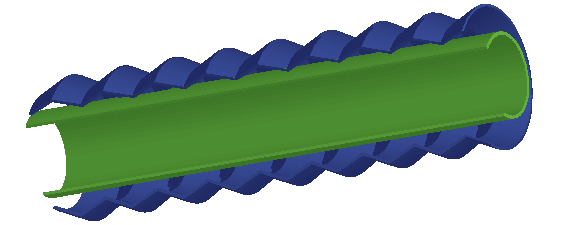
\includegraphics[width=6in]{fast-chamber.pdf}
  \caption[Illustrating a fast subchamber residing within another subchamber.]
{\label{f:fast} A ``fast'' subchamber (green), which uses fewer cross-sections to describe
it, resides within another ``slow'' (blue) subchamber with many cross-sections. The fast
subchamber enables \srthree to speed up tracking. The two subchambers have been cut in
the illustration to better show the geometry.}
  \end{figure}

%------------------------------------------------------------------
\section{Fast and Slow Subchambers}
\label{s:fast}

When a subchamber has many cross-sections (which can easily happen when a multi-section
(\sref{s:multi.sec}) is used), the computation time for photon tracking may become large
due to the necessity of stopping the photon at each cross-section to check whether the
photon has crossed the subchamber boundary. This can be ameliorated by defining an
associated ``fast'' subchamber with only a few cross-sections that is contained withing
the ``slow'' subchamber with the large number of cross-sections as illustrated in
\fig{f:fast}.

As explained in \sref{s:track}, when a photon is tracked that is contained in both a slow
and an associated fast subchamber, \srthree can ignore the slow subchamber and track the
photon through the fast subchamber until the photon exits the fast subchamber. Tracking
will be quicker since there will be fewer cross-sections to stop the photon at.

To associate two subchambers as a fast/slow pair, a \vn{fast_slow} namelist instance is used.
The syntax of this namelist is:
\begin{example}
  &fast_slow
    fast = "<fast_subchamber_name>"
    slow = "<slow_subchamber_name>"
  /
\end{example}
A \vn{fast_slow} namelist instance establishes a single association. So to make multiple
associations, multiple \vn{fast_slow} namelist instances need to be used.

A subchamber can have multiple associated slow or fast subchambers. A subchamber can also
have an associated fast subchamber and an associated slow subchamber although in practice
this is to be avoided since it will, if anything, slow down tracking.

A fast subchamber may extend beyond the slow subchamber it is associated with. The entire
vacuum chamber is the union of all subchambers including the fast ones. That is, in terms
of defining the vacuum chamber, fast subchambers are no different than the slow ones or
the ``normal'' subchambers that do not have any fast or slow associations.

%------------------------------------------------------------------
\section{Lattices with Branches}
\label{s:lat.branch}

  \begin{figure}
  \centering
  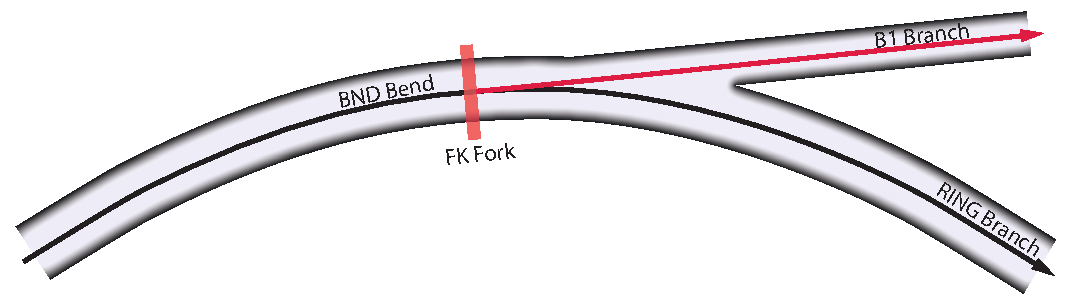
\includegraphics[width=6in]{branch-line.pdf}
\caption{Branch line illustration. Here a branch line named \vn{b1} is connected to the
root branch, named \vn{ring}, via a fork element named \vn{fk}.}
  \label{f:branch.line}
  \end{figure}

To describe things like injection lines or a ring attached to a X-ray beam line, a lattice will
have multiple ``branches''. [See the Bmad manual\cite{b:bmad} for more details on lattice
branches.] By default, subchambers will be associated with the ``root'' branch (branch 0).
A \vn{subchamber_branch} namelist is used to associate a subchamber with a given
branch. The form of this namelist is:
\begin{example}
  &subchamber_branch
    subchamber_name = <name>
    branch_name = <name-or-index>
  /
\end{example}
The \vn{subchamber_name} is the name of the subchamber to be associated and
\vn{branch_name} is name or index of the associated branch.

As an example, consider the following lattice:
\begin{example}
  parameter[E_tot] = 1e9
  bnd: sbend, l = 2.0, g = 0.1
  fk: fork, superimpose, ref = bnd, offset = -0.2, to_line = b1
  dd: drift, l = 3
  ring: line = (..., b, ...)
  b1: line = (dd, ...)
  b1[geometry] = open
  use, ring
\end{example}
This lattice is illustrated in \fig{f:branch.line}.  This lattice has two branches. The
root branch is named \vn{ring} and this branch contains a bend called \vn{bnd}.
Superimposed upon \vn{bnd} is a \vn{fork} element called \vn{fk} which forks to the second
branch called \vn{b1}.

The wall file for this example is:
\begin{example}
  &place section = 0.0,  "", "main:sdef" /
  &place section = 2.0,  "", "main:sdef" /
  &place section = 0.0,  "", "x_wall:sdef" /
  &place section = 3.0,  "", "x_wall:sdef" /

  &shape_def
    name = "sdef"
    v(1) =    0.01,    0.01
  /

  &subchamber_branch
    subchamber_name = "x_wall"
    branch_name = "b1"
  /
\end{example}
There are two subchambers. One subchamber named \vn{main} is, by default, associated with
the root branch -- \vn{ring}. The other subchamber, named \vn{x_wall}, is associated with
the \vn{b1} branch.

%------------------------------------------------------------------
\section{Subchamber Surface Interpolation} 
\label{s:wall}

Once a set of subchamber cross-sections have been defined, the
cross-section of the subchamber at a given longitudinal position is
computed using linear interpolation. 

For a given subchamber, and at a given $s$ position, the $r, \theta$ coordinate system in the
transverse $x, y$ plane is defined with respect to an origin $\bfr_O(s)$ given by a linear
interpolation of the origins of the cross-sections to either side of the given $s$ position. Let
$s_1$ denote the position of the cross-section just before $s$ and $s_2$ denote the position of the
cross-section just after $s$. Let $\bfr_{01}$ be the $(x_0, y_0)$ origin defined for the cross
section at $s_1$ and $\bfr_{02}$ be the $(x_0, y_0)$ origin defined for the cross section at
$s_2$. Then
\Begineq
  \bfr_O(s) = (1 - \stilde) \, \bfr_{01} + \stilde \, \bfr_{02}
\Endeq
where 
\Begineq
  \stilde \equiv \frac{s - s_1}{s_2 - s_1}
\Endeq

Let $r_{c1}(\theta)$ and $r_{c2}(\theta)$ be the radiusus of the
sub-section boundary as a function of $\theta$ for the cross-sections
at $s = s_1$ and $s = s_2$ respectively. The sub-section boundary
$r_c(\theta, s)$ at any point $s$ between $s_1$ and $s_2$ is then
defined by the equation
\Begineq
  r_c(\theta, s) = (1 - \stilde) \, r_{c1}(\theta) + \stilde \, r_{c2}(\theta)
\Endeq

A photon at $(r,\theta, s)$ is inside the subchamber if
\Begineq
  r < r_w(\theta, s)
\Endeq

%------------------------------------------------------------------
\section{Subchamber Surface and Patch Elements}
\label{s:patch}

A \vn{patch} element, which shifts the reference coordinate system
complicates the calculation of where a photon hits the wall. The Bmad
manual has a full explanation but the essential factor is that, since
the reference orbit is discontinuous in a patch, to avoid a
discontinuity in the subchamber surface, wall interpolation is done using
the global reference system. This can lead to non-intuitive behavior
when the region between two wall sections contains both a bend and a
patch since, without the patch, the center of the subchamber follows the
curved reference orbit but with the patch the subchamber surface center
follows a straight line between the wall sections.

To avoid this non-intuitive behavior, if a region between wall sections
contains both a patch and a bend, extra sections will be added to
eliminate this situation.

To simplify matters, \srthree does not allow wall cross-sections to be
defined whose longitudinal position overlaps any \vn{patch} element.

%------------------------------------------------------------------
\section{Chamber Surface Reflectivity}
\label{s:surface}

By default, the photon reflectivity of the vacuum chamber wall is based on the
reflectivity of a 10 nm C film on an Al substrate. This default can be changed by setting
the following parameters in the master input file (\sref{s:master}):
\begin{example}
    surface_reflection_file
    surface_roughness_rms
    roughness_correlation_len 
\end{example}

If the chamber wall is made up of sections of differing material,
additional surface types can be defined using \vn{surface_def}
namelists in the chamber wall file. The syntax for this namelist is
\begin{example}
  &surface_def
    reflectivity_file = "<file_name>"
  / 
\end{example}
\vn{reflectivity_file} is a file that specifies the surface reflectivity as 
explained in (\sref{s:reflect.file}).

To associate a particular material with a particular region of the
chamber wall, the optional \vn{surface} variable is set for the
\vn{place} namelist (\sref{s:sub.chambers}), at the downstream
(maximal $s$) end of the region of interest. The syntax is:
\begin{example}
  &place
    section = ...
    surface  = "<name>", <is_local>
  /
\end{example}
The \vn{<name>} here must match the \vn{name} in the surface reflectivity file The two
exceptions are if \vn{<name>} is set to
\begin{example}
  ABSORBER              ! Case sensitive
  PHANTOM               ! Case sensitive
\end{example}
The \vn{ABSORBER} setting makes the surface a perfect absorber. The \vn{PHANTOM} setting
is for surfaces where, if \vn{filter_phantom_photons} (\sref{s:master.example}) is True,
if a photon hits the phantom surface, it is not counted in the final statistics. This is
useful for situations like simulating an X-ray beam pipe where, for the purposes of the
simulation, the pipe is terminated at some point and photons intersecting the end of the
pipe are not to be considered to have hit a wall but rather to have safely gone through to
the experimental end station. Effectively, photons intersecting a phantom wall is treated
as any other photon that fails a filter test (\sref{s:master.example}). Note that,
independent of the setting of \vn{filter_phantom_photons}, a phantom surface acts like a
perfect absorber. That is, there are never any reflections from a phantom surface.

If \vn{<is_local>} is \vn{True}, then the surface material only spans the region from the
previous cross-section to this one. If \vn{<is_local>} is \vn{False} or not present, the
surface material spans from the closest previous cross-section where there is a
\vn{surface} variable set to this cross-section.  If a \vn{place} instance refers to a \vn{multi_section}
(\sref{s:multi.sec}), and \vn{<is_local>} is \vn{True} then the material
only spans the multi_section region.

{\em \vn{Note:}} For any given region with finite area of the vacuum chamber wall, if there are
multiple subchambers whose surfaces overlap the region, it is important to make sure that the surface
types of these subchambers are all the same since, for a photon striking this region, which
subchamber is used to compute the surface properties is ill-defined. As an example, consider Figure
\vn{f:vac-chamber}. The overlap between the two subchamber surfaces are the two lines where the
subchamber surfaces intersect. Since the overlap has zero area, it is OK to have the two subchambers
have different surface types.

If a region of the vacuum chamber wall is defined by multiple
subchambers (that is, multipole subchamber surfaces coincide in this region), which
subchamber is used to select the surface type can vary from photon to photon. Therefore,
it is important to make sure that for any given point on the vacuum chamber wall, that the
local surface type is the same for all subchambers that have walls that coincide with the
point in question.

Example:
\begin{example}
  &place section = 0.0, "elliptical", ... /
  &place section = 1.0, "elliptical", ... /
  &place 
    section = 3.0, "elliptical", ... /
    surface = "ss", True
  /
  &place
    section = 5.0, "multi_section:ms", ...
    section = "ni", True
  /
  &place
    section = 7.0 "elliptical", ...
    surface = "cu"
  /
  &place 10.0 section = ... /

  &surface_def
    name = "ss"
    reflectivity_file = "ss_burnished.reflect"
  /
\end{example}
Assuming the multi_section spans the region from 5~meters to 6~meters,
the materials associated with different regions of the chamber are:
\begin{example}
 S_begin    Surface    S_end
 -------    -------    -----
   0.0         cu       1.0
   1.0         ss       3.0
   3.0         cu       5.0
   5.0         ni       6.0
   6.0         cu       7.0
   7.0       default   10.0
\end{example}

%------------------------------------------------------------------
\section{Old Wall Format}
\label{s:old.wall}

Originally, \srthree did not have the concept of subchambers. That is,
there was only one chamber and that chamber was allowed to be concave.
This was problematical, as discussed above, and motivated the
development of the subchamber concept. This section discusses the old
format to facillitate conversion from the old format to the new.
Example of the old format:
\begin{example}
  &section_def section =   0.0, "arc_std", "elliptical", 0.045, 0.025 /
  &section_def section =  74.3, "Near_IR"  "gen_shape:dipole_shape",  /
  &section_def section =  82.9, "wig1",    "rectangular", 0.045, 0.025 /
  &section_def section =  91.1, "IR1",     "rectangular", 0.045, 0.025, 
                                                       -1, -1, 0.08, 0.01 /
\end{example}

The \vn{<section_id>} can have one of five values:
\begin{example}
  elliptical                   
  rectangular                  
  gen_shape:<shape_name>       
  multi_section:<shape_name>   
\end{example}
Historically, the \vn{elliptical} and \vn{rectangular} shapes where
developed first. The \vn{gen_shape} was developed later and is a
generalization of the original two shapes. The \vn{elliptical} and
\vn{rectangular} cross-sections are explained in the next
section. \vn{Gen_shape} is explained in the
section after and \vn{multi_section} is explained in the section
after that.


\begin{figure}[tb]
\begin{center}
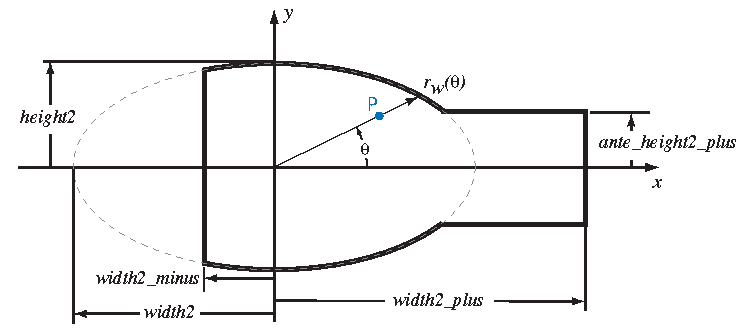
\includegraphics[width=6in]{chamber.pdf}
\caption{Example vacuum chamber cross-section for an \vn{elliptical} 
chamber with an antechamber on the $+x$ side of the chamber and an
aperture on the $-x$ side.}
\label{f:chamber}
\end{center}
\end{figure}

An example \vn{elliptical} cross-section is shown in
\fig{f:chamber}. The format for an \vn{elliptical} or \vn{rectangular}
cross-section is
\begin{example}
  &section_def 
    section = <s>, <section_name> <section_id>, <width2>, <height2>, <width2_plus>, 
              <ante_height2_plus>, <width2_minus>, <ante_height2_minus> /
    surface = "<surface_name>", <is_local>
\end{example}
The first five parameters -- \vn{<s>}, \vn{<section_name>}
\vn{<section_id>}, \vn{<width2>}, and \vn{<height2>} -- must be
specified. Values for the other parameters are optional and default to
the ``unset'' value of -1.

The optional \vn{surface} variable is explained in \sref{s:surface}.

For \vn{elliptical} or \vn{rectangular} shapes, the
parameters needed to specify the chamber are:
\begin{example}
  <s>                   ! Longitudinal position
  <section_name>        ! Descriptive Name of the cross-section.
  <section_id>          ! Either "elliptical" or "rectangular"
  <width2>              ! Half width ignoring antechamber.
  <height2>             ! Half height ignoring antechamber.
  <width2_plus>         ! Distance from pipe center to +x side edge.
  <ante_height2_plus>   ! Antechamber half height on +x side of the wall
  <width2_minus>        ! Distance from pipe center -x side edge.
  <ante_height2_minus>  ! Antechamber half height on -x side of the wall
\end{example}

For both \vn{"rectangular"} and \vn{"elliptical"} shapes, \vn{<width2>}
and \vn{<height2>} define the half-height and half-width of the shape.

Antechambers on the $+x$ side and/or $-x$ side of the chamber can be
added to the basic shape. On the $+x$ side, an antechamber is formed
if the \vn{<ante_height2_plus>} parameter is set to a positive value. If
\vn{<ante_height2_plus>} is set to a positive value, as shown in
\fig{f:chamber}, the parameter \vn{<width2_plus>} specifies the
horizontal distance from the chamber center to the far end of the $+x$
side antechamber. In this case, the value of \vn{<width2_plus>} must be
large enough so that the antechamber far wall does not stick back into
the basic shape. For a rectangular shape, this translates to
\vn{<width2_plus>} being larger than \vn{<width2>}. Similarly, if
\vn{<ante_height2_minus>} is set to a positive value, an antechamber is
formed on the $-x$ side.  In this case, \vn{<width2_minus>} is the
(positive) horizontal distance from the chamber center to the far end
of the $-x$ antechamber.

If \vn{<ante_height2_plus>} is not set, a set of \vn{<width2_plus>}
defines an aperture on the $+x$ side of the chamber. In this case, the
value of \vn{<width2_plus>} must be less than the value of
\vn{<width2>}. Similarly, if \vn{<ante_height2_minus>} is not set, a set of
\vn{<width2_minus>} defines an aperture on the $-x$ side of the chamber.
A $-x$ aperture is shown in \fig{f:chamber}.

Example:
\begin{example}
  ! Anything outside the namelists is ignored.
  &section_def section =   0.0, "arc_std", "elliptical", 0.045, 0.025 /
  &section_def section =  82.9, "wig1",    "rectangular", 0.045, 0.025 /
  &section_def section =  91.1, "IR1",     "rectangular", 0.045, 0.025, 
                                                         -1, -1, 0.08, 0.01 /
\end{example}


Prescription for converting:
\begin{enumerate}
\item If there are \vn{\&section_def} namelists that use rectangular or elliptical shapes. 
      That is, no "gen_shape:..." is present then the appropriate \vn{\&shape_def} namelists will have to be created. 
      If the shape is not convex, the shape will need to be split into subchambers.
\item rename: "gen_shape:..." to "..." in \vn{\&section_def} namelists. 
      If the shape is not convex, the shape will need to be split into subchambers.
\item If present, remove ``ix_vertex_ante1'' and ``ix_vertex_ante2'' lines from \vn{\&gen_shape_def}.
      To get the correct antechamber absorbtion, use a separate subchamber for the antechamber regions.'
\item rename: ``\vn{\&section_def}'' to ``\vn{\&place}''.
\item rename: ``\vn{\&gen_shape_def}'' to ``\vn{\&shape_def}''.
\item If a \vn{shape_def} has a name that has a colon ``:'', replace this by some other character.
\end{enumerate}

%------------------------------------------------------------------
\chapter{Photon Tracking \& Reflections}

%------------------------------------------------------------------
\section{Photon Tracking}
\label{s:track}

\begin{figure}[tb]
\begin{center}
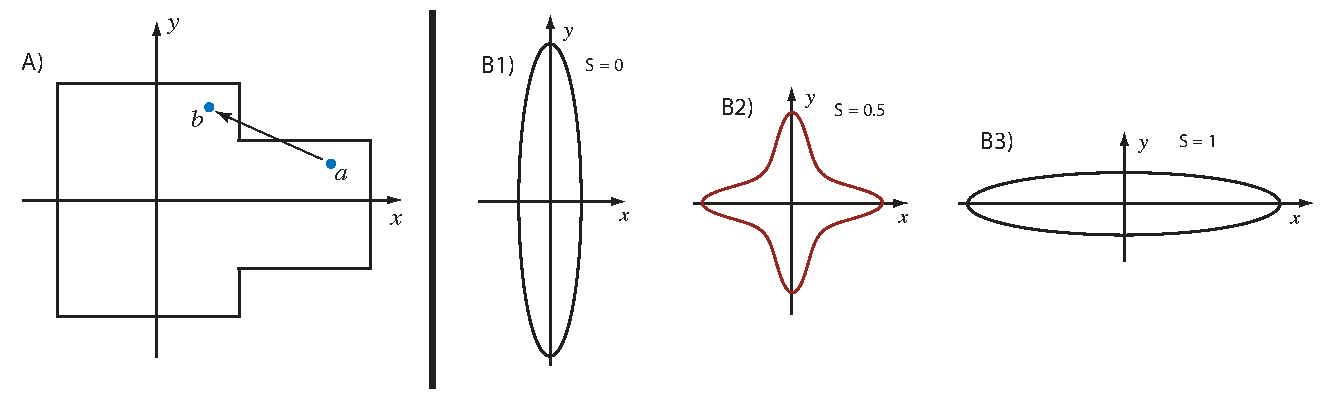
\includegraphics[width=6in]{chamber-problem.pdf} \caption{A) A convex cross-section can
lead to problems with linear interpolation since it is assumed that if the beginning and
ending points of a step are inside the subchamber the entire track is inside the
subchamber. The track shown violates this assumption.  B) With linear interpolation,
convex cross-sections are not a guarantee that intermediate cross-sections are convex. B1
and B3 are the defined cross sections at $s = 0$ and $s = 1$ respectively. These cross
sections are ellipses with 5:1 aspect ratio. The interpolated cross-section B2 at $s =
0.5$ is seen to be concave.}  \label{f:convex-chamber}
\end{center}
\end{figure}

When a photon is created, \srthree checks to see if the photon is within any
subchamber. If the photon is not within any subchamber, that is, if it is outside the
vacuum chamber wall, \srthree will generate an error message if the number of photons that
have been generated up to this point exceed \vn{num_ignore_generated_outside_wall}. If
the generated photon is within the vacuum chamber wall, the phton is ``associated'' with
one of the subchambers that it is within.  The photon will be tracked through the
associated subchamber until it reaches the edge of the subchamber.

When the photon reaches the edge of the associated subchamber it is going through,
\srthree checks if there is a suitable alternative subchamber to switch association to. A
suitable subchamber is any subchamber that the photon is within or a subchamber where the
photon is at the edge and has velocity directed inward.

If there is a suitable alternative, \srthree will associate the photon with the
alternative subchamber and keep tracking until the photon gets to the edge of this
subchamber.  This process of reassociating the photon to a second subchamber when the
photon reaches the edge of the current associated subchamber will continue until there is
no suitable alternative. At this point the photon has hit the vacuum chamber wall.

When tracking a photon through its associated subchamber, \srthree can ignore all other
subchambers since, by definition, if the phton is inside its associated subchamber, it
is inside the vacuum chamber.

The exception to the above process happens when the subchamber associated with a photon
itself has an associated ``fast'' chamber (\sref{s:fast}). In this case, \srthree, while
tracking through the slow subchamber, will periodically check to see if the photon is also
within the fast subchamber, if it is, the photon's associated subchamber will be switched
to the fast subchamber.

Photons are tracked in ``steps''. A step consists of propagating a photon from it's
current position to some new position that is a certain distance away. The length to
propagate the photon in a given step is determined by a number of factors. The maximum
length for a step is set by the input parameters
\begin{example}
  sr3d_params%ds_track_step_max
  sr3d_params%dr_track_step_max
\end{example}
These set longitudinal (\vn{%ds_track_step_max}) and transverse (\vn{%dr_track_step_max})
distances. Additionally, a single step will always be terminated at, and never cross over,
a defined cross-section plane of the subsection associated with the photon. Steps will
also be terminated at the boundaries of bend magnets and at the point in a bend where a
trajectory is closest to the center of the bending radius.

After a step, the new photon position is checked to see if it is still
inside the associated subchamber. If it is not, the point where it has crossed
the subchamber surface is calculated via a root finding algorithm.

If the new photon position is inside the associated subchamber, there is still the
question as to whether the photon trajectory between the beginning step point and the end
step point is inside the subchamber. \srthree assumes that the subchamber is ``locally
convex''. That is, given the two end points of a step with points inside the subchamber,
it is assumed that the line drawn between these two points never touches or goes outside
the subchamber. This locally convex assumption will be true if every cross-section
$r_w(\theta, s)$ for fixed $s$ is convex where $s$ is in the range of longitudinal $s$
positions covered by the step in question.

\srthree assumes that if the beginning and ending points of a step are inside the
subchamber, the entire track is inside the subchamber. This assumption my be violated if
the cross-section of a subchamber is concave as illustrated in
Fig.~\ref{f:convex-chamber}A.  Furthermore, even if two defined cross-sections are
themselves convex, an intermediate cross-section can be concave as shown in
Fig.~\ref{f:convex-chamber}B. 

A subchamber ``region'' is the volume of the subchamber between two adjacent
cross-sections. The total subchamber volume is thus the sum of all the regions of the
subchamber. Since \srthree always limits steps so that the beginning and ending points of
a step cannot be in different regions, there is no problem with \srthree failing to detect
photons crossing the chamber wall as long as each region indivdually is convex in
shape. This is true even if the subchamber considered as a whole is not convex.

How much of a problem the possibility that \srthree will not
detect some photons leaving and then entering the chamber will, of course, depend upon the
specifics of the chamber geometry and what is being calculated. One way to test if this is
a problem this is to reduce the track step length limits:
\begin{example}
    sr3d_params%ds_track_step_max
    sr3d_params%dr_track_step_max
\end{example}
This will reduce the possibility of mis-tracking at the cost of
increased computation time. If the results do not change significantly
when the track limits are reduced, this is good evidence that the 
results are valid.

Notice that if all the subchambers are convex there will be no problem even if the union
of the subchambers -- which defines the entire vacuum chamber -- is concave. To put it
another way, given a concave vacuum chamber, if the vacuum chamber can be constructed
using a number of convex subchambers, there will be no problem with \srthree not detecting
photons leaving and entering the vacuum chamber in a single step.

%------------------------------------------------------------------
\section{photon\_start\_input\_file}
\label{s:photon.start}

The \vn{photon_start_input_file} file is used to specify starting positions
for the photons. This is done typically for debugging purposes.

The \vn{photon_start_input_file} file contains a number of
\vn{\&start} namelists. One for each photon starting position. The
format for a \vn{\&start} namelist is:
\begin{example}
  &start
    orbit%vec = <x>, <vx/c>, <y>, <vy/c>, 0.0, <vz/c>  ! Photon position
    orbit%s   = <s>   ! Longitudinal distance from start of lattice.   
    orbit%p0c = <ev>  ! Photon energy
    ran_state = <random_state_struct>
    random_seed = <num>
    ix_branch = <num>  ! Lattice branch index to start photon in. Default is 0.
  /
\end{example}
The fifth component of \vn{orbit%vec} is not used and should be set to zero.
The \vn{orbit%s} component is the longitudinal distance
from the start of the lattice.  If needed, The \vn{ran_state} and
\vn{random_seed} parameters can be used to initialize the random number
generator.

The magnitude of the velocity, $\sqrt{v_x^2+v_y^2+v_z^2}/c$ must be 1.

%------------------------------------------------------------------
\section{Surface Reflection File}
\label{s:reflect.file}

A surface reflectivity file is used to redefine the default chamber
wall surface reflectivity (By setting \vn{surface_reflection_file}
in the master input file (\sref{s:master})) or to define the
surface reflectivity for a particular wall material (\sref{s:surface}).

The probability for a photon reflecting from a wall is dependent upon
the grazing angle and the photon energy. For a given graze angle and
photon energy, there are two reflection probabilities called
\vn{p_reflect} and \vn{rel_p_specular} These determine the
probabilities that the photon will be reflected either diffusely or
specularly, or that the photon will be absorbed. In particular
\begin{example}
  probability of absorption          = 1 - p_reflect
  probability of reflection          = p_reflect
  probability of specular reflection = p_reflect * rel_p_specular
  probability of diffuse reflection  = p_reflect * (1 - rel_p_specular)
\end{example}
Generally, \vn{p_reflect} will be near unity at small
grazing angles and fall off with increasing angle. At the smaller
photon energies ($E \lesssim 100 \, \mbox{eV}$), the reflection
probabilities will still be substantial at grazing angles of
10~degrees or more. At the larger photon energies ($E \gtrsim 1000 \,
\mbox{eV}$), The reflection probabilities are quite peaked and are
small above a few degrees.

\vn{rel_p_specular} is given by Equations (1) and (2) in Reference
\cite{b:synrad3d} and so \vn{rel_p_specular} is not specified in a
reflection file.

In the reflection probability file, the reflection probability \vn{p_reflect} is
specified at a number of different angles and energies. \srthree will
interpolate as needed. Reflections probabilities are specified over
some energy range from $E_{min}$ to $E_{max}$. If a photon has an
energy below $E_{min}$, reflection probability is taken to be the same
as the probability at $E_{min}$. If a photon has an energy $E_p$ that
is above $E_{max}$, it is assumed that the reflection probability is
the same as the reflection probability at energy $E_{max}$ and angle
$\theta_g(\mbox{eff}) = \theta_g * E_p / E_{max}$ where $\theta_g$ is the
photon grazing angle. If $\theta_g(\mbox{eff})$ is grater than 90~degrees,
90~degrees is used for $\theta_g(\mbox{eff})$.

For specifying the reflection probabilities, the energy range from
$E_{min}$ to $E_{max}$ is broken up into a number of ``tables'' each
covering some energy interval. The tables are ordered in increasing
energy so that table 1 starts from $E_{min}$ and the last table goes
up to $E_{max}$. The energy intervals for the tables abut one another
so that the upper energy of one table is the lower energy of the next.
Each table specifies the reflection probabilities at a number of
energies $E_i, i = 1, \ldots, N_E$ and a number of grazing angles
$\theta_j, j = 1, \ldots, N_\theta$. The energies $E_i$ must be
equally spaced and in ascending order but the grazing angles
$\theta_j$ do not only have to be in ascending order with $\theta_1 =
0$ and $\theta_{N_\theta} = 90$. Except for the restriction that the
energy intervals of the tables abut one another, the tables are
independent in the sense that, for example, the spacing between the
$E_i$, the particular $\theta_j$ chosen, etc. can vary from table to
table. The reason for having multiple tables is for compactness. That
is, the particular choice of the spacing between the $E_i$ and the
particular $theta_j$ chosen can be optimized for each energy interval
to give the maximum accuracy with the least amount of input data.

The probability file must start with a namelist named \vn{general}
that specifies the number of tables and roughness numbers. Example:
\begin{example}
  &general
    name = "ConCu"      ! Case sensitive
    description = "50um C layer on Cu substrate"
    n_table = 5    ! 5 tables
    surface_roughness_rms      = 200e-9   ! meters
    roughness_correlation_len  = 5.5e-6   ! meters
  /
\end{example}
The \vn{name} parameter is used to identify the surface in the vacuum chamber wall file
(\sref{s:wall.file}). The \vn{description} parameter is an optional description string
that \srthree prints when plotting reflectivity curves.

Next, each table is specified in turn starting from the table for the
lowest energy interval. A table is specified starting with a
\vn{table} namelist. There are two different syntaxes that can be used here
An example of the first syntax is:
\begin{example}
  &table
    energy_min    =  600 ! eV
    energy_max    = 1400 ! eV
    energy_delta  =   20 ! eV
    angles =  0.0, 0.4, 0.8, 1.0, 1.5, 2.0, 3.0, 4.0, 90.0
  /
\end{example}
In this example, the energy range is from 600 eV to 1400 eV in steps of 20 eV and the
reflection probability is specified at 9 different grazing angles (in degrees). Angles
must start at 0 and end at 90 degrees.

An example of the second \vn{table} namelist syntax is:
\begin{example}
  &table
    energies = 7, 10, 31, 45
    angles =  0.0, 0.4, 0.8, 1.0, 1.5, 2.0, 3.0, 4.0, 90.0
  /
\end{example}
In this example, the angle points are the same but the energy points are specified point
by point.  This second syntax is useful when the reflection data is not evenly spaced. 

After the \vn{table} namelist, for each energy ``row'', \vn{p_reflect} is
specified by a \vn{row} namelist. Example:
\begin{example}
  &row
    ix_row = 2   ! 620 eV
    p_reflect =  1.00, 0.941, 0.882, 0.852, 0.771, 0.669, 0.514, 0.056, 0.0
  /
\end{example}
There must one \vn{row} namelist for each energy value in the table. For this example
there would be 41 \vn{row} namelists. The \vn{row} namelists must be in order of
increasing energy and each \vn{row} namelist has a \vn{ix_row} component which must be set
to \vn{1} for the first \vn{row} namelist, \vn{2} for the second, etc. \srthree uses
\vn{ix_row} as a sanity check when reading in the table. The \vn{p_reflect} component of
the \vn{row} namelist give the reflection probabilities at the $N_\theta$ angle points.

There must be no gaps between the energy ranges of the tables. That is, the lowest energy
of one table must be at most the highest energy of the previous table. On the other hand,
it is permitted for the energy ranges of the tables to overlap.

%------------------------------------------------------------------
\chapter{Output Files} 

%------------------------------------------------------------------
\section{Main Output File}
\label{s:main.out}

The \vn{dat_file} (whose name is specified in the master input file (\sref{s:master})) is
divided into two parts. the top part essentially echos the information provided in
the main input file. It looks like:
\begin{example}
  # photon_number_factor    =  8.155E-01
  # num_photons_generated   = 123    ! Total including filtered photons.
  # I0_tot                  = 0.34   ! I0 radiation integral for the ring
  # ix_ele_track_start      = 103
  # ix_ele_track_end        = 104
  # photon_direction        = 1
  # num_photons             = 10
  # num_photons_per_pass    = -1
  # random_seed             = 123456
  # lattice_file            = "../tao/examples/cesr/lat.bmad"
  # photon_start_input_file = ""
  # wall_file               = "synrad3d.wall"
  # dat_file                = "synrad3d.dat"
  # chamber_end_geometry    = ""
  # ds_step_min             =  1.000E-02
  ... etc ...
\end{example}

The first line gives the \vn{photon_number_factor} which is computed via the formula
\Begineq
  \text{photon_number_factor} = 
    \frac{5 \, \sqrt{3} \, e^2 \, I_0}{4 \, \pi \, \epsilon_0 \, \hbar \, c \, N_{sim}}
\Endeq
where $N_{sim}$ is the number of photons generated in the
simulation run, and $I_0$ is the synchrotron radiation integral
\Begineq
  I_0 = \int_{emit} ds \, \gamma_0 \, g(s)
\Endeq
with $g(s)$ being the bending strength (equal to $1/\rho$, with $\rho$ being the bending radius), and the
integral is done over the region where photons are emitted in the simulaiton.

\vn{photon_number_factor} is related to $N_{\gamma}$, the total number of photons per
beam particle emitted in one revolution in the actual machine via
\Begineq
  \text{photon_number_factor} = \frac{N_\gamma}{N_{sim}}
\Endeq
Thus, if $N_r(\text{sim})$ is the number of simulated photons absorbed in a particular region,
the actual number of photons $N_r(\text{actual})$ absorbed in this region per beam particle per turn
is
\Begineq
  N_r(\text{actual}) = \text{photon_number_factor}  \cdot N_r(\text{sim})
\Endeq

The second part of the file is a table. Each row is the data for one photon. Only photons
that pass the filter tests are shown. The table looks like:
\begin{example}
   1       2  6.981783E+02   -0.000221    0.001255    0.000052   ... etc.
   2       1  4.705803E+03    0.000605    0.001255    0.000050   ... etc.
   3       2  6.883773E+02    0.001430    0.001255    0.000048   ... etc.
   4       2  3.463312E+02    0.002255    0.001255    0.000046   ... etc.
   5       1  2.104224E+01    0.003080    0.001255    0.000043   ... etc.
   6       2  1.393605E+02    0.003904    0.001254    0.000041   ... etc.
   7       5  1.979004E+01    0.004729    0.001254    0.000039   ... etc.
   8       2  4.288703E+02    0.005553    0.001253    0.000037   ... etc.
   9      12  1.493411E+01    0.006377    0.001253    0.000034   ... etc.
  10       2  1.297799E+02    0.007200    0.001252    0.000032   ... etc.
\end{example}

The columns of the file are:
\begin{example}
  1:      Photon index number.
  2:      The number of times the photon has struck the vacuum 
              chamber wall including the final hit. 
  3:      The photon energy (in eV).
  4-9:    Initial photon position $x$, $V_x/c$, $y$, $V_y/c$, $s$, $V_s/c$.
  10      Index of the lattice branch where the photon was created
  11-16:  Final photon position
  17:     sin(graze_angle). 0 = Grazing incidence, 1 = perpendicular incidence.
  18:     Photon travel length
  19:     Photon longitudinal travel length - beam travel length 
                                                       in the same time period.
  20:     Index of the lattice branch where the photon is absorbed.
  21:     Lattice element index where photon is absorbed.
  22:     Lattice element type (Eg: quadrupole, etc.) where photon is absorbed.
  23:     sub-chamber name where photon is absorbed.
\end{example}  

$x$ is the horizontal position (direction along the
local normal to the closed orbit, in the bend plane, zero on the
closed orbit, positive to the outside of the machine, ), $y$ is the
vertical position (direction perpendicular to the bend plane, zero on
the closed orbit, positive up), and $s$ is the longitudinal position
(direction tangent to the closed orbit, zero at the beginning of the
lattice, positive in the direction of motion of the beam).

%------------------------------------------------------------------
\section{Wall Hit Output File}
\label{s:wall.hit.file}

If the switch \vn{wall_hit_file} is non-blank, an additional output file is generated,
which contains more detailed information on where photons are hitting the vacuum chamber
wall. Example:
\begin{example}
  1     0       0.0     -0.0008    0.0000     67.7857       0.0000   ... etc.
  1     1     698.2      0.0450   -0.0002     70.5150       0.0323   ... etc.
  1     2     698.2     -0.0393   -0.0138     71.2168      -0.1152   ... etc.
  2     0       0.0     -0.0007    0.0000     67.8515       0.0000   ... etc.
  2     1    4705.8      0.0450    0.0001     70.5782       0.0322   ... etc.
  3     0       0.0     -0.0006    0.0000     67.9172       0.0000   ... etc.
  3     1     688.4      0.0450    0.0004     70.6414       0.0322   ... etc.
  3     2     688.4     -0.0450   -0.0020     71.0368      -0.2197   ... etc.
  4     0       0.0     -0.0005    0.0000     67.9829       0.0000   ... etc.
  4     1     346.3      0.0450   -0.0003     70.7046       0.0322   ... etc.
  4     2     346.3     -0.0450   -0.0014     71.2347      -0.1643   ... etc.
  5     0       0.0     -0.0004    0.0000     68.0487       0.0000   ... etc.
  5     1      21.0      0.0450    0.0003     70.7678       0.0321   ... etc.
\end{example}
The columns of this file are:
\begin{example}
  1:     photon_index  
  2:     wall_hit_index  
  3:     photon_energy             ! When wall_hit_index = 0 this is 0]
  4-6:   (x, y, s)                 ! Coordinates of photon at wall
  7:     ix_branch                 ! Index of lattice branch where photon is.
  8-10:  (vx, vy, vs)              ! Velocity before bounce.
  11-13: (vx, vy, vs)              ! Velocity after bounce.
  14-16: (perp_x, perp_y, perp_z)  ! Wall perpendicular.
  17:    cos_perp_in               ! Cos of photon incoming direction wrt wall.
  18:    cos_perp_out              ! Cos of photon outgoing direction wrt wall.
  19:    reflectivity              ! Reflectivity coef.
  20:    sub-chamber               ! Subchamber name where photon hits.
\end{example}
The \vn{photon_index} is the same index as in the main output file. The
\vn{wall_hit_index} starts at 0 for the emission point and increases up to the value for
\vn{n_wall_hits} in the main file.  The \vn{photon_energy} will be the same as in the main
file.

Columns 4 through 6 give the coordinates of the photon where it strikes the wall.  except
that the entry for wall_hit_index = 0 gives the emission point coordinates.

Columns 8 through 10 gives the velocity of the photon just before it bounces and columns 11
through 13 gives the velocity just after it bounces (or what would be its velocity if it
does not get absorbed).

Columns 14 through 16 give the perpendicular vector to the wall at the point of photon
impact.

Columns 17 and 18 give the cosine of the angle between the wall perpendicular and the
photon velocity just before and just after the bounce. 0 = photon velocity parallel to wall,
$\pm 1$ = photon velocity perpendicular to wall.

Column 18 gives reflectivity which is a function of the type of surface and the photon
orientation with respect to the wall.

If the photon is ``adsorbed'' due to reflections being disallowed, columns 10 and
higher will be zero.

In the example given above, the first photon is absorbed after reflecting once.
and the second photon is not reflected at all being absorbed on the first hit.

Note: If the beam emittances are zero, photons will be generated on
the central orbit. If there are no steerings powered, the central
orbit will be the zero orbit and in this case all photons will start
with $x$ = $vx$ = $y$ = 0.

Note: Since the $(x,y,s)$ coordinates are curved in bend elements, the photon trajectory
in $(x,y,s)$ coordinates is not, in general, a straight line between hit points. For more
accurate plotting, a \vn{photon_track_file} (\sref{s:photon.track.file}) should be
generated. Caution: \vn{photon_track_file}s are over an order of magnitude larger than
\vn{wall_hit_file}s.

%------------------------------------------------------------------
\section{Photon Track Output File}
\label{s:photon.track.file}

A photon track file records the photon position after each propagation step.  A photon
track file is generated if the \vn{photon_track_file} parameter is set to something that
is not blank in the master input file (\sref{s:master}). 

This file is useful for plotting photon trajectories since it records intermediate points between
points where the photon hits a wall. However, if a large number of photons are generated, this
file can be very large.

Example track file output:
\begin{example}
  1   1  -0.00082    0.00005    67.78576   0      0.00000    0.00000    0.00000
  1   1   0.04500   -0.00022    70.51507   0      0.03230   -0.00010    0.99947
  1   1  -0.03930   -0.01381    71.21681   0     -0.11528   -0.01921    0.99314
  2   4  -0.00074    0.00005    67.85150   0      0.00000    0.00000    0.00000
  2   4   0.04500    0.00012    70.57826   0      0.03227    0.00002    0.99947
  3   5  -0.00065    0.00005    67.91725   0      0.00000    0.00000    0.00000
  3   5   0.04500    0.00046    70.64145   0      0.03224    0.00015    0.99948
  3   5  -0.04500   -0.00206    71.03689   0     -0.21972   -0.00623    0.97554
  4   7  -0.00057    0.00005    67.98299   0      0.00000    0.00000    0.00000
  4   7   0.04500   -0.00037    70.70463   0      0.03221   -0.00015    0.99948
  4   7  -0.04500   -0.00149    71.23479   0     -0.16439   -0.00208    0.98639
  5   9  -0.00049    0.00005    68.04873   0      0.00000    0.00000    0.00000
  5   9   0.04500    0.00039    70.76781   0      0.03218    0.00012    0.99948
\end{example}
The columns of this file are
\begin{example}
  1:     Photon index  
  2:     Generated photon index.
  3-5:   (x, y, s)                 ! Coordinates of photon 
  7:     ix_branch                 ! Index of lattice branch photon is in.
  7-9:   (vx, vy, vs)              ! Velocity of the photon
\end{example}

Column 1 gives the photon index which gives a count of the photons that have been tracked
and passed the filter restrictions. Only photons that have passed the filter restriction have
their tracks recorded in the file. Thus the photon index numbers will be consecutive.

Column 2 gives the photon generation index. Each tracked photon is given a unique
generation index starting from 1. Thus for the example above, photons with generation
index 1, 4, 5, 7 and 9 passed the filter tests and thus are present in the file. Photons
with generation index 2, 3, 6, and 8 did not pass the filter tests and are not shown in
the file.

Columns 3 through 5 give the position of the photon.

Columns 7 through 9 gives the velocity of the photon.

%------------------------------------------------------------------
\chapter{Test Modes}
\label{s:test}

Test modes are used to generate diagnostic data files. tests are also useful for generating data for
plotting reflection statistics.Test modes are specified using the \vn{-test <what>} option on the
command line (\sref{s:run}).
\begin{example}
  -test monte_carlo_reflection ! \sref{s:test.monte}
  -test specular_reflection    ! \sref{s:test.specular}
  -test diffuse_probability    ! \sref{s:test.diffuse}
\end{example}

These test modes are explained below. In all cases, the \vn{synrad3d_parameters} namelist in the
master input file (\sref{s:master.example}) is ignored and instead another namelist is read in from
the master input file as specified in the documentation below.

%------------------------------------------------------------------
\section{Monte Carlo Reflection Test}
\label{s:test.monte_carlo}

The \vn{monte_carlo_reflection} test mode, invoked by using the \vn{-test mone_carlo_refleciton} on
the command line (\sref{s:run}). The output of this test are a number of lines recording the
direction of the outgoing scattered photon under the conditions where the photon energy and incoming
graze angle are fixed.

The parameters used for the test are read in from the master input file specified on the command
line (\sref{s:run}). The namelist used for the input parameters for the reflection test is called
\vn{reflection_test}.  Example:
\begin{example}
  &reflection_test
    surface_reflection_file      = ""      ! Reflection probability file
    graze_angle_in               = 0.12    ! Incident grazing angle in radians.
    energy                       = 100     ! Photon energy in eV
    surface_roughness_rms        = -1      ! Roughness for diffuse scattering.
    roughness_correlation_len    = -1      ! Roughness correlation length.
    n_photons                    = 1000    ! Number of reflections simulated
    random_seed                  = 0       ! Random number seed.
    include_specular_reflections = F       ! Diffuse reflections only?
    output_file                  = ""      ! Blank => Use default name.
  /
\end{example}

The \vn{surface_reflection_file} specifies the reflection probability file to be used. If no file is
specified then the default surface is used (\sref{s:dflt.reflect}).

The \vn{graze_angle_in} is the incident grazing angle in radians and \vn{energy} in the photon
energy in eV. \vn{n_photons} are the number of reflections to simulate, and \vn{output_file} is the
name of the output data file. The default data file name is "test_monte_carlo_reflection.dat". The
other parameters are explained in \sref{s:master}.

If the \vn{include_specular_reflections} parameter is set to \vn{True}, specular reflection is
allowed. Otherwise only diffuse reflections are simulated. The default is \vn{False}.

The \vn{surface_roughness_rms} parameter sets the surface roughness. If negative then the roughness
specified by the surface is used.

The \vn{roughness_correlation_len} parameter sets the surface roughness correlation. If negative
then the correlation specified by the surface is used.

\vn{random_seed} is the random number seed used in by the random number generator. If set to 0, the
system clock will be used. That is, if set to 0, the output results will vary from run to run.

The output contains a header with the input parameters followed by
\vn{n_photon} lines. Each line is of the form:
\begin{example}
  theta_out  phi_out
\end{example}
where \vn{theta_out} is the grazing angle of the reflected photon in radians.  \vn{theta_out} = 0
means the photon is traveling parallel to the surface. The \vn{phi_out} angle is the azimuthal angle
in radians with zero \vn{phi_out} indicating that the incident ray, the surface normal, and
reflected rays are in the same plane.

%------------------------------------------------------------------
\section{Specular Reflection Test}
\label{s:test.specular}

Specular reflection test mode (\sref{s:run}), invoked using the \vn{-test specular_reflection}
option on the command line, is used for studying specular (angle in = angle out) reflections from a
given set of photon initial conditions using the chamber wall specified by the \vn{wall_file}
parameter in the Master Input file.  Each photon is allowed a single specular reflection and the
initial and final photon position and velocity are recorded in the output file.

The parameters used for the test are read in from the master input file specified on the command
line (\sref{s:run}). The namelist used for the input parameters for the reflection test is called
\vn{specular_reflection_test}.  Example:
\begin{example}
  &specular_reflection_test
    photon_start_input_file = "photon.start"  ! Photon starting positions
    lattice_file            = "lat.bmad"      ! Lattice file
    wall_file               = "synrad3d.wall" ! Wall definition file
    output_file             = ""     ! Default is "test_specular_reflection.dat"
  /
\end{example}

The \vn{photon_start_input_file} is the file of initial photon positions. The format of this file is
given in \vn{s:photon.start}.  Note that for the specular test, values for the photon energy and the
random number generator state in the initial photon position file do not affect the results and do
not have to be set. Also: The if the magnitude of the velocity $\sqrt{v_x^2+v_y^2+v_z^2}/c$ is not
too far off from 1 then \srthree will renormalize so that $\sqrt{v_x^2+v_y^2+v_z^2}/c$ will be 1.

\vn{lattice_file} give the name of the lattice.  The lattice file format may be the Bmad format or,
if the \vn{lattice_file} string is prefixed by \vn{``xsif::''}, may be in xsif format. See the Bmad
manual for more details.

The \vn{wall_file} gives the name of the vacuum chamber will definition file. See \sref{s:wall.file}
for more details.

The \vn{output_file} gives the name of the output data file.  See \sref{s:wall.hit.file} for details
of the syntax for this file.

%------------------------------------------------------------------
\section{Diffuse Probability Test}
\label{s:test.diffuse}

The \vn{diffuse_probability} test mode, invoked using the \vn{-test diffuse_probability}
option on the command line, creates a table of diffuse reflection probabilities.

The parameters used for the test are read in from the master input file specified on the command
line (\sref{s:run}). The namelist used for the input parameters for the reflection test is called
\vn{diffuse_probability_test}.  Example:
\begin{example}
  &diffuse_probability_test
    surface_reflection_file   = ""      ! Reflection probability file
    graze_angle_in            = 0.12    ! Incident grazing angle in radians.
    energy                    = 100     ! eV
    surface_roughness_rms     = -1      ! Roughness for diffuse scattering.
    roughness_correlation_len = -1      ! Roughness correlation length.
    prob_normalization        = "1"     ! Probability normalizaton.
    output_file               = ""      ! Blank => Use default name.

    row_type                 = "energy" ! Table row type.
    row_min                  = 10       ! Min row value
    row_max                  = 1000     ! Max row value
    row_n_pts                = 101      ! Number of row lines.
    row_log_scale            = T        ! Use log scale?
    row_values               = 0.001, 0.003, 0.01 ! Alternative way to
                                        ! specify row values.

    graze_angle_out_min      = 0.001    ! Minimal value in radians
    graze_angle_out_max      = 0.010    ! Maximal value
    graze_angle_out_n_pts    = 10       ! Number of graze angle columns.
    graze_angles_out         = 0.001, 0.003, 0.01 ! Alternative way to
                                        ! specify outgoing graze angles.
  /
\end{example}

The output is a table. Each row shows the reflection probability for different values of the parameter
specified by \vn{row_type}. Possible \vn{row_type} settings are:
\begin{example}
  "azimuth_angle_out" ! Outgoing azimuth angle of the photon.
  "energy"            ! Photon energy rows.
  "roughness"         ! Surface roughness.
  "correlation"       ! Surface correlation length.
  "graze_angle_in"    ! Incoming photon graze angle.
\end{example}

The output table has a number of columns. The first column is an index number from 1 to the number
of rows in the table.  The second column is the value of what \vn{row_type} is being used. The other
columns will be the diffuse reflection probability for a certain value of outgoing graze angle. 

If the \vn{row_type} is set to \vn{"azimuth_angle_out"}, the rows will be the outgoing azimuth angle
$\phi$ of the photon. In this case, the probabilities shown in the table will be the probability
$P(x, \phi)$ of scattering a photon with outgoing orientation $x$ and $\phi$ where $x =
\sin(\theta_{\text{g,out})$ with $\theta_{\text{g,out}$ is the outgoing graze angle (see Equation
A138 of \cite{b:prab}). 

If \vn{row_type} is set to anothing else but \vn{"azimuth_angle_out"}, the probabilities shown in
the table will be the probability $P_x(x)$ which is the scattering probability integrated over
$\phi$ (see Equation A140 of \cite{b:prab}).

The values used for the parameter specified by \vn{row_type} can be set in one of two ways.
One way is to specify an explicit list of values using the \vn{row_values} parameter. Example:
\begin{example}
  row_values = 0.001, 0.003, 0.01
\end{example}
The alternative way is to set \vn{row_min}, \vn{row_max}, \vn{row_n_pts} and \vn{row_log_scale}. This
will create \vn{row_n_pts} number of rows with the \vn{row_type} parameter ranging from \vn{row_min} 
to \vn{row_max}. The points will be evenly spaced if \vn{row_log_scale} is set to \vn{False} and will
be evenly spaced on a log scale if \vn{row_log_scale} is set to \vn{True}. Note: If \vn{row_n_pts} is
positive then this alternative is used. Otherwise the values from \vn{row_values} are used.

Similar to specifying row values, the column values for the outgoing graze angle can be set either
by setting \vn{graze_angles_out} to a list of values or by setting \vn{graze_angle_out_min},
\vn{graze_angle_out_max}, and \vn{graze_angle_out_n_pts}.

The \vn{surface_reflection_file} specifies the reflection probability file to be used. If no file is
specified then the default surface is used (\sref{s:dflt.reflect}).

The \vn{graze_angle_in} parameter sets the incoming graze angle but is ignored if \vn{row_type} is
set to "graze_angle_in".

The \vn{energy} parameter sets the photon energy but is ignored if \vn{row_type} is set to "energy".

The \vn{surface_roughness_rms} parameter sets the surface roughness. If negative then the roughness
specified by the surface is used. This parameter is ignored if \vn{row_type} is set to "roughness".

The \vn{roughness_correlation_len} parameter sets the surface roughness correlation. If negative
then the correlation specified by the surface is used. This parameter is ignored if \vn{row_type} is
set to "correlation".

The \vn{prob_normalization} parameter sets how the displayed probabilities are normalized. Possible
settings are:
\begin{example}
  "1" 
  "reflect"
  "all"
\end{example}
A setting of "1" means that the displayed probability integrated over all outgoing angles (and
keeping everything else fixed) is 1. That is, absorption and specular reflection probabilities are
ignored. A setting of "relect" means that the integrated probability will be the probability of
being diffusely reflected relative to the probability of being reflected and not absorbed. That is,
abosrbtion is ignored.  Finally, a setting of "all" means that the integrated probability will be
the probability of being diffusely reflected taking into account both absorbtion and specular
reflection probabilities.

The default file name for the output data file is \vn{test_diffuse_probability.dat}.


%------------------------------------------------------------------
\appendix
\chapter{Spline Fit of the Diffuse Probability Function}
\label{c:spline}

The diffuse scattering theory used in \srthree is discussed by Dugan and Sagan\cite{b:prab} (D\&S)
with one change pertaining to how the integrated diffuse probability function $C_x(x)$ (D\&S
Eq.~A144) is evaluated. 

In D\&S, $C_x$ was evaluated using a Chebyshev fit to the probability function $P_x(x)$ in the
interval $[0,1]$. While this gives good results with relatively rough surfaces where $P_x$ is fairly
broad smooth function, the fit will be poor when the surface roughness is small and $P_x$ is a
peaked function with the peak centered at $x = y$. [That is, the diffuse reflection becomes specular
like (angle out = angle in) in the limit where the surface is smooth.] The reason why the Chebyshev
fit becomes poor when $P_x$ becomes peaked is due to the fact that a Chebyshev fit is a polynomial
fit and it takes a polynomial of large degree to fit a peaked function well.

As a replacement, a spline fit with adaptive point selection was implemented. The Akima spline
used\cite{b:akima} has the advantage of locality (the calculated slope at a knot point is only
affected by the local knot points around it) and the ability to better handle large changes in slope
since an Akima spline does not try to maintain a continuous second derivative. The adaptive point
selection is used to better fit peaked functions. The basic idea here is to find at what knot point
the estimated integrated area error is largest and then to add knot points to either side of this
knot point. The integrated area error at a given knot point is estimated by the difference between
the integrated area from the previous knot point to the next knot point using the spline fit and the
integrated area as calculated from a cubic fit to the three knot points (previous point, point under
consideration and the next point). Adding points is stopped when the estimated error for the total
integral is below some fraction of the total integral.

%------------------------------------------------------------------
% \appendix
\chapter{Default Reflectivity Tables.}
\label{s:dflt.reflect}

  \begin{figure}
  \centering
  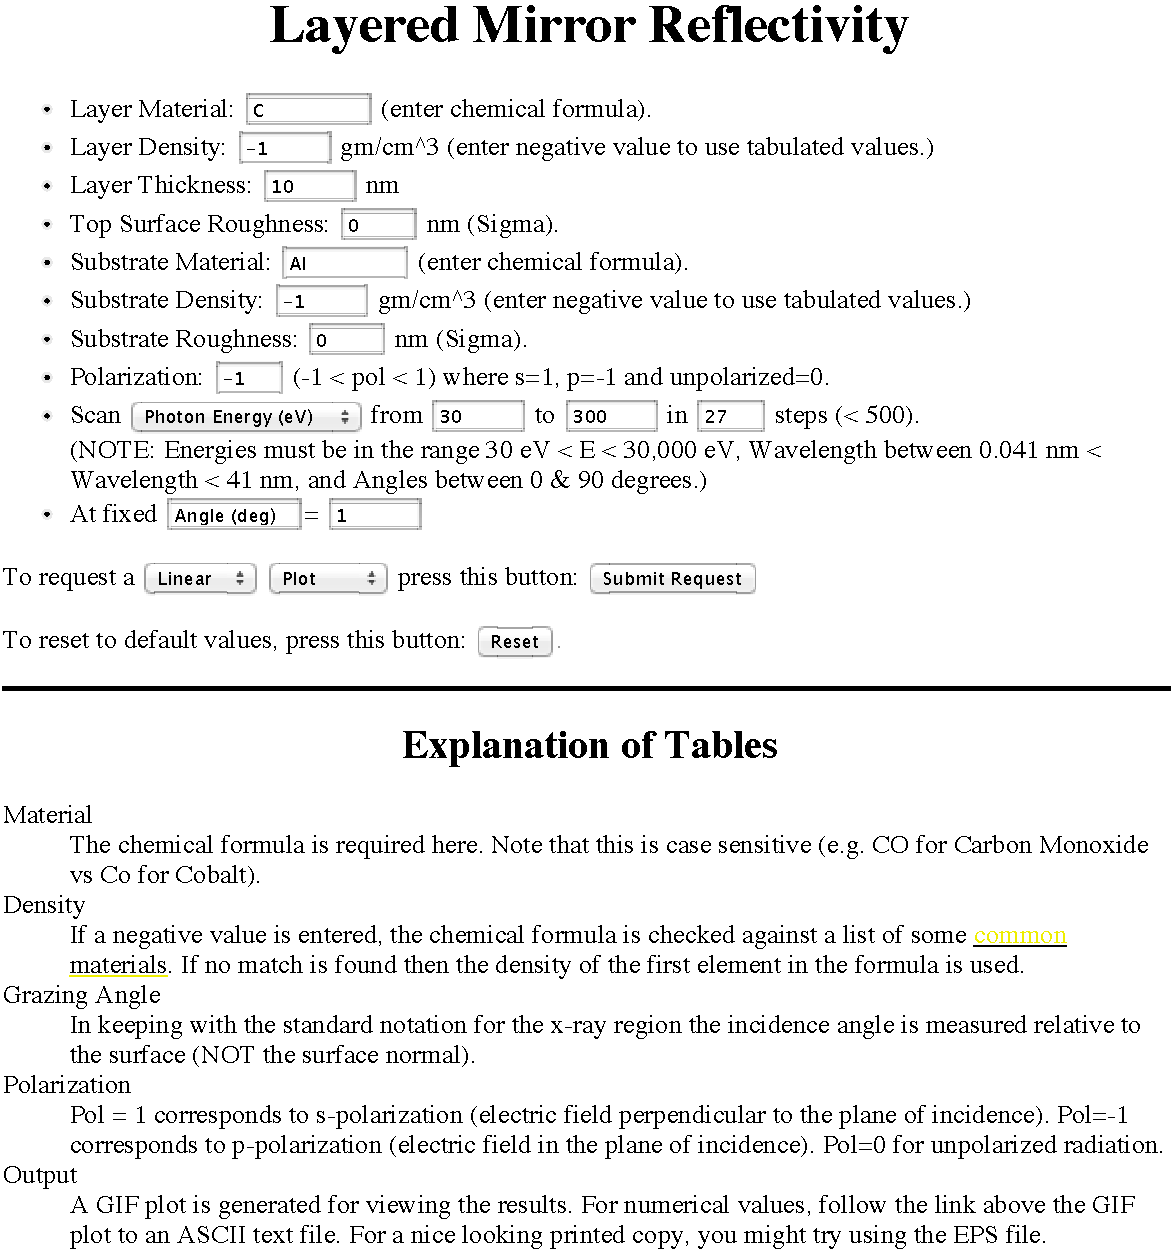
\includegraphics[width=5in]{Layered_Mirror_Reflectivity.pdf}
  \caption[Input parameters for the default reflectivity curves.]
  {
Input parameters for the default reflectivity curves used by \srthree.
  }
\label{f:reflect}
  \end{figure}

The default reflectivity used by \srthree is based on a calculation
for a 10 nm C film on an Al substrate. Figure~\ref{f:reflect} shows
the parameters used to generate the reflectivity tables. The tables
are from the LBNL X-ray data base found at:
\begin{example}
  http://henke.lbl.gov/optical_constants/layer2.html
\end{example}

The polarization choice, $P=-1$, was made since this corresponds to the
polarization direction of the direct synchrotron radiation striking
the chamber surface, on the first encounter. It is probably not really
correct for subsequent scatterings. However the polarization
dependence of the reflectivity is not very strong.

The default surface roughness for diffuse scattering is 200~nm and the
default surface roughness correlation length is 5.5~$\mu$m. These
values can be modified by setting \vn{surface_roughness_rms} and
\vn{roughness_correlation_len} in the master input file
(\sref{s:master}).

%------------------------------------------------------------------
\chapter{Customizing Synrad3D}
\label{c:custom}

\srthree is designed so that custom code, created by you, can be used for generating photons. This
custom code is compiled with the \srthree library to create a custom executable.

%------------------------------------------------------------------
\section{Setup}
\label{s:custom.setup}

Creating a custom version of \srthree involves creating custom code that is put in a directory that
is distinct from the \vn{bsim} directory which is the directory that contains the standard \srthree
code files.

\textbf{It is important to remember that the code in the \vn{bsim} directory is not to be modified.
This ensures that, as time goes on, and as \srthree is developed, changes to the code in the
\vn{bsim} directories will have a minimal chance to break your custom code.} If you do
feel you need to change something in the \vn{bsim} directory, please seek help first.

To setup a custom \srthree version do the following:
  \begin{enumerate}
  \item
Establish a base directory in which things will be built. This directory can have any name. Here we
will call this directory \vn{ROOT}. This base directory can be located anywhere. It is recommended that
if you have a local Bmad \vn{Distribution}, that you keep the base directory separate from the \vn{Distribution}
  \item
Make a subdirectory of \vn{ROOT} that will contain the custom code. This directory can have any
name.  Here this directory will be called \vn{synrad3d_custom}.
  \item
Copy the files from the directory \vn{bsim/synrad3d/custom} to \vn{ROOT/synrad_custom}. The
\vn{bsim} directory is part of the Bmad Distribution package. If you do not know where to find it, ask your
local Guru where it is. 

There are three files in the \vn{bsim/synrad3d/custom} directory. One file is a template file for 
creating custom code called
\begin{example}
  photon_init_custom.f90
\end{example}
There is documentation in this file on how to customize it. To have this custom routine called, the
\vn{photon_start_input_file} (\sref{s:master.example}) must be set to ``\vn{CUSTOM}''.

The other two files are CMake\footnote{CMake is a program used for
compiling code} script files which do not have to be modified. These files are
\begin{example}
  CMakeLists.txt
  cmake.custom_synrad3d
\end{example}
These scripts are setup to make an executable called \vn{custom_synrad3d}. This name can be changed
by modifying the \vn{cmake.custom_synrad3d} file.
  \item
Copy the file \vn{bsim/synrad3d/synrad3d.f90} to \vn{ROOT/synrad3d_custom}. This file should not
be modified.
  \item
Go to the \vn{ROOT/synrad3d_custom} directory and use the command \vn{mk} to create the
executable 
\begin{example}
    \vn{ROOT/production/bin/custom_synrad3d}. 
\end{example}
Similarly, the command \vn{mkd} will create a debug executable 
\begin{example}
    \vn{ROOT/debug/bin/custom_synrad3d}
\end{example}
	\end{enumerate}
A debug executable only needs to be created if you a debugging the code.

%------------------------------------------------------------------
\begin{thebibliography}{9}

\bibitem{b:bmad}
D. Sagan,
``Bmad: A Relativistic Charged Particle Simulation Library''
Nuc.\ Instrum.\ \& Methods Phys.\ Res.\ A, {\bf 558}, pp 356-59 (2006).

\bibitem{b:henke} 
B.L. Henke, E.M. Gullikson, and J.C. Davis. X-ray
interactions: photoabsorption, scattering, transmission, and
reflection at E=50-30000 eV,=1-92, Atomic Data and Nuclear Data
Tables Vol. 54 (no.2), 181-342 (July 1993) {\tt
http://henke.lbl.gov/optical\_constants/}

\bibitem{b:beckmann}
P.~Beckmann \& A.~Spizzichino, \emph{The Scattering of Electromagnetic Waves
  from Rough Surfaces}, Pergamon Press, New York (1963).

\bibitem{b:ogilvy}
J.~A. Ogilvy, \emph{Theory of Wave Scattering from Random Rough Surfaces},
  Hilger, Bristol (1993).

\bibitem{b:prab}
G. Dugan and  D. Sagan, ``Simulating Synchrotron Radiation in Accelerators Including 
Diffuse and Specular Reflections'', Phys. Rev. Accel. Beams, {\bf 20}, 020708, (2017).

\bibitem{b:synrad3d}
 G.Dugan and D.Sagan, ``SYNRAD3D: Photon Propagation and Scattering Simulations,''
`` INFN-LNF/INFN-Pisa/CERN-LER/EuCARD-AccNet Joint Workshop on Electron-Cloud Effects (ECLOUD12)'', (2012).

\bibitem{b:mehne}
N. Mahne et. al., ``Experimental Determination of ECLOUD Simulation Input
Parameters for DA$\Phi$NE'', EuroTev-Report-2005-013 (2005).

\bibitem{b:jackson} J. D. Jackson,
\emph{Classical Electromagnetism}, third edition, Wiley, New York (1999)

\bibitem{b:akima}
H. Akima, 
``A New Method of Interpolation and Smooth Curve Fitting Based on Local Procedures,'' 
J.ACM, vol. 17, no. 4, pp. 589-602, (1970).

\end{thebibliography}
\end{document}  
